\section{Neural Networks and Deep Learning}

%%%%%%%%%%%%%%%%%%%%%%%%%%%
%%%%%%%%%%%%%%%%%%%%%%%%%%%
%%%%%%%%%%%%%%%%%%%%%%%%%%%
%%%%%%%%%%%%%%%%%%%%%%%%%%%
%%%%%%%%%%%%%%%%%%%%%%%%%%%
\subsection{Introduction}

A neural network is a ML model inspired by the network of biological neurons in our brains.

NNs are versatile, powerful, and scalable.
Consequently, they frequently outperform other ML techniques on very large and complex problems.
NNs are at the very core of Deep Learning.

\textbf{Threshold Logic Units (TLUs)} are the building block of neural networks (i.e. the neurons):
\begin{itemize}
\vspace{-4.0mm}

\item
First, they perform a weighted sum of the inputs, $z = \sum w_i x_i$

\item
\vspace{-2.0mm}
Then they apply an \textit{activation function} to that sum, $h_{\boldsymbol{w}}(\boldsymbol{x}) = \phi(z)$, and output the result.\newline
\begin{figure}[ht]
\centering
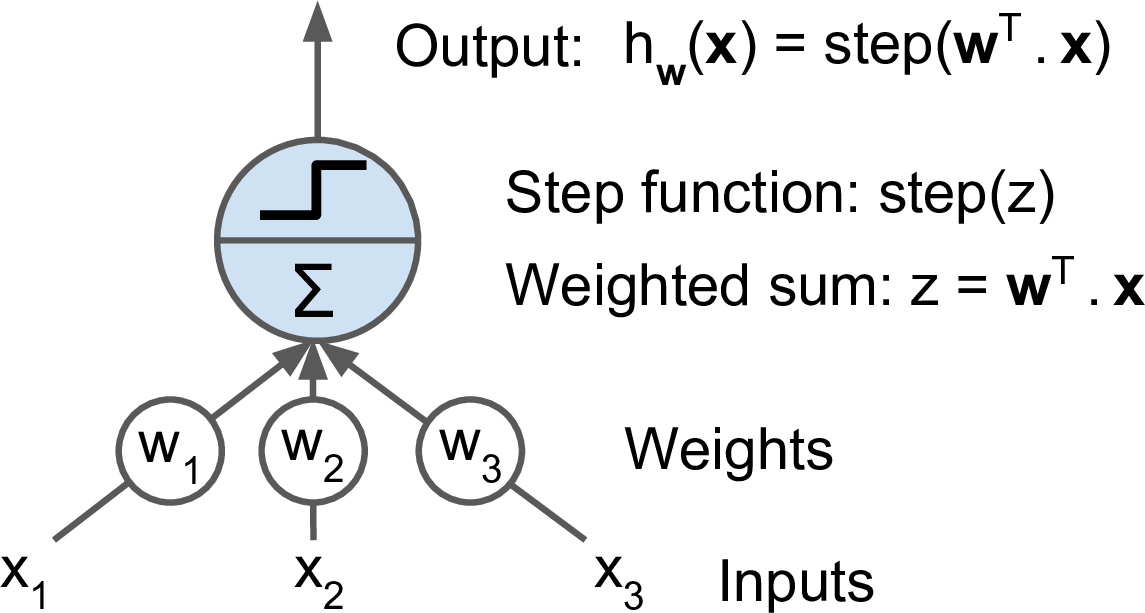
\includegraphics[width=0.50\textwidth]{./images/TLU.png}
\end{figure}

\item
\vspace{-2.0mm}
Traditionally, the activation function was a heavyside step function.
However, in order to perform Gradient Descent on a NN,
a differentiable function was needed instead.\newline
- The default has become the Rectified Linear Unit function: ReLU(z) = max(0,z)\newline
- The logistic function and hyperbolic tangent function are also popular choices.
\end{itemize}
\vspace{-2.0mm}


\textbf{Multilayer Perceptrons (MLPs)} are composed of multiple TLUs as depicted in the diagram.\newline
\textit{The bias neurons are shown, but usually they are implicit.}
\begin{figure}[ht]
\centering
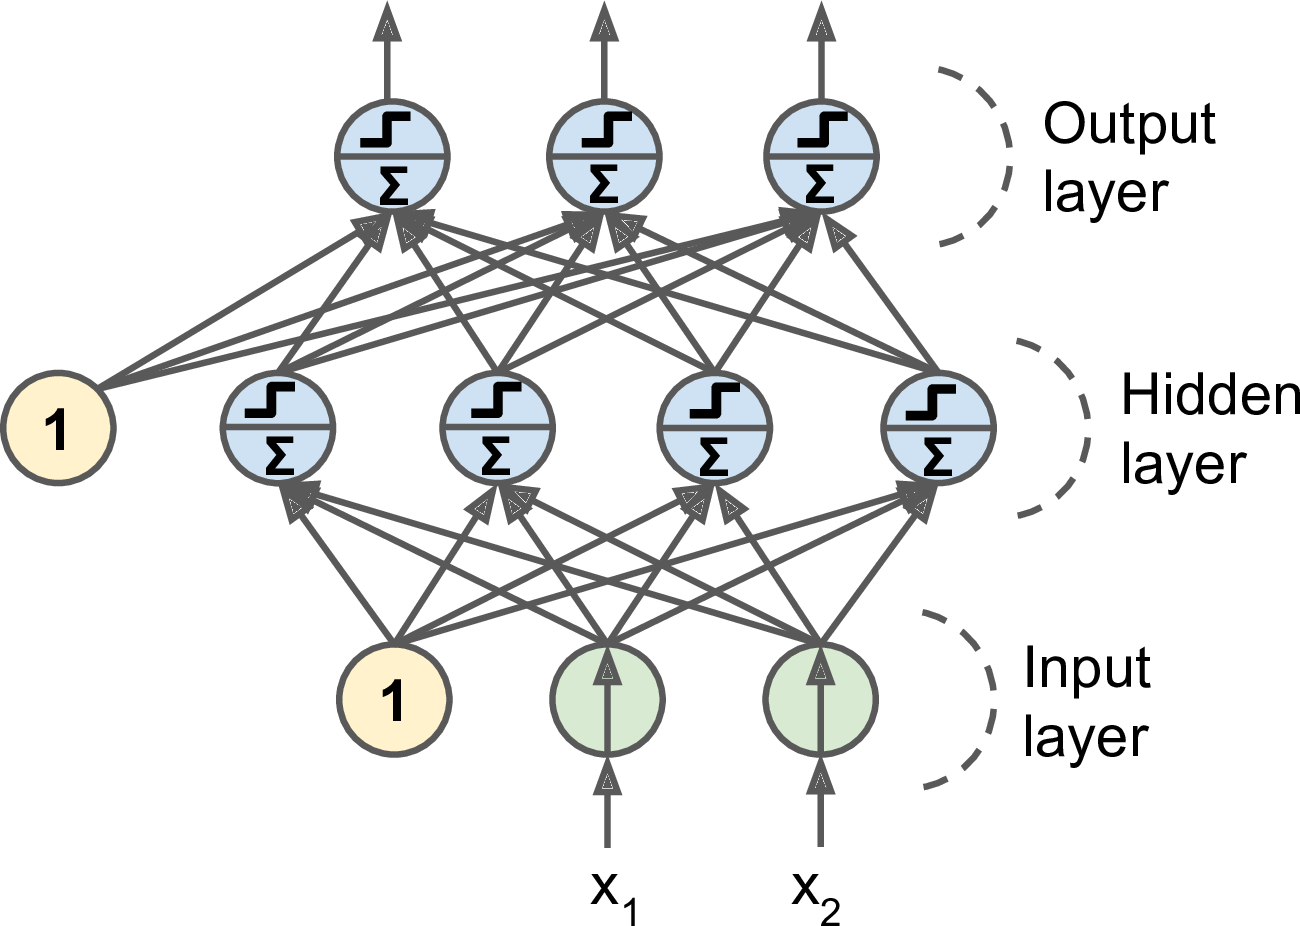
\includegraphics[width=0.50\textwidth]{./images/MLP.png}
\end{figure}

\vspace{-6.0mm}
\begin{itemize}
\item
When there's a deep stack of hidden layers, it is called a \textit{deep neural network (DNN)}.
\item
\vspace{-2.0mm}
Layers close to the input layer are called the \textit{lower layers}\newline
Layers close to the output layer are called the \textit{upper layers}.
\item
\vspace{-2.0mm}
When all the neurons in a layer are connected to every neuron in the previous layer,\newline
the layer is called a \textit{fully connected layer} or a \textit{dense layer}.
\item
\vspace{-2.0mm}
The signal flows only in one direction $=$ \textit{feedforward neural network (FNN)}.
\item
\vspace{-2.0mm}
Without the activation functions, all you would get is a linear model!
\end{itemize}

\newpage
\textbf{Training NNs: Backpropagation}.\newline
In just two passes through the network (one forward, one backward)
the backpropagation algorithm is able to compute the gradient of the network's error
with regard to every single model parameter (i.e. the connection weights),
allowing Gradient Descent to be used to train the NN.

\vspace{-5.0mm}
\begin{itemize}
\item
It handles one mini-batch at a time. The bigger the batch size, the more memory required.

\item
\vspace{-2.0mm}
\textit{The forward pass}.
Each mini-batch is passed through the network.
The output of every neuron is computed and preserved (for every instance in the mini-batch).

\item
\vspace{-2.0mm}
The network's output error is measured.

\item
\vspace{-2.0mm}
\textit{The reverse pass}.
The error gradient across all the connection weights is measured
by propagating the error gradient backward through the network.

\item
\vspace{-2.0mm}
An \textbf{iteration} = one forward-backward pass using one mini-batch.\newline
An \textbf{epoch} = one forward-backward pass of \textit{all} the training set examples.\newline
If you have 2000 training examples, and your batch size is 500...\newline
$\rightarrow$ then it will take 4 iterations to complete 1 epoch.

\item
\vspace{-2.0mm}
It is important to randomly initialize all the hidden layer's connection weights.\newline
This breaks the symmetry and allows backpropagation to train a diverse team of neurons.

\end{itemize}

\textbf{Regression MLPs: Summary}

\begin{tabular}{ |l|l| } 
\hline
Hyperparameter & Typical value \\ 
\hline
Number of input neurons & One per input feature \\ 
Number of hidden layers & Depends on the problem, but typically 1 to 5\\ 
Number of neurons per hidden layer & Depends on the problem, but typically 10 to 100\\ 
Hidden layer activation function & ReLU or SELU\\
Number of output neurons & 1 per prediction dimension\\
Output activation function & In general None (can output any range of values)\\
 & ReLU/softplus (for a positive output contraint)\\
 & Logistic/tanh (for a bounded output contraint)\\
Loss function & Typically MSE (mean squared error)\\
 & Maybe MAE (mean absolute error) when there's lots of outliers\\
\hline
\end{tabular}

\textbf{Classification MLPs: Summary}

\begin{tabular}{ |l|l| } 
\hline
Hyperparameter & Typical value \\ 
\hline
Number of input neurons & One per input feature \\ 
Number of hidden layers & Depends on the problem, but typically 1 to 5\\ 
Number of neurons per hidden layer & Depends on the problem, but typically 10 to 100\\ 
Hidden layer activation function & ReLU or SELU\\
Number of output neurons & 1 (for binary classification)\\
 & 1 per label (for multilabel binary classification)\\
 & 1 per class (for multiclass classification)\\
Output activation function & Logistic (for binary classification)\\
 & Softmax (for multiclass classification)\\
Loss function & Cross entropy\\
\hline
\end{tabular}

\newpage
The architecture of an MLP for multiclass classification:

\begin{figure}[ht]
\centering
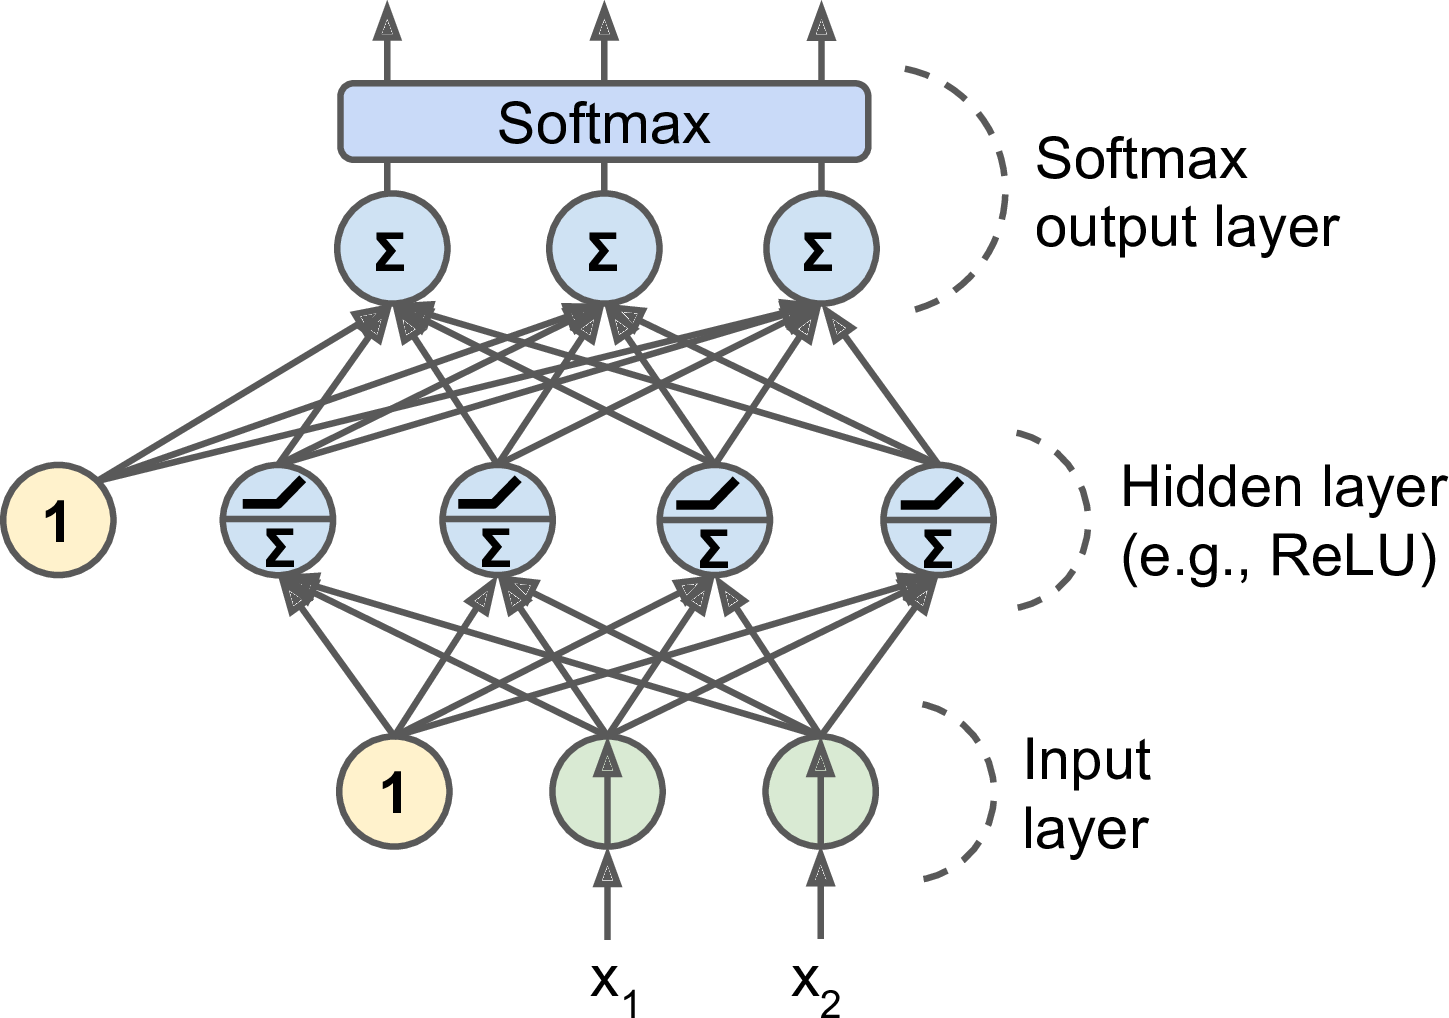
\includegraphics[width=0.50\textwidth]{./images/MLP_classification.png}
\end{figure}

%%%%%%%%%%%%%%%%%%%%%%%%%%%
%%%%%%%%%%%%%%%%%%%%%%%%%%%
%%%%%%%%%%%%%%%%%%%%%%%%%%%
%%%%%%%%%%%%%%%%%%%%%%%%%%%
%%%%%%%%%%%%%%%%%%%%%%%%%%%

\subsection{Implementing MLPs with Keras}

The following code creates a classification MLP with:
\vspace{-5.0mm}
\begin{itemize}
\item
An input layer with 784 neurons, where each instance is a $28*28$ array.
\vspace{-3.0mm}
\item
Two hidden layers (with 300 and 100 neurons, respectively).\newline
Both layers use the ReLU activation function.\newline
All the layers are connected sequentially.
\vspace{-3.0mm}
\item
10 exclusive classification outputs.
\end{itemize}

\vspace{-2.0mm}
\texttt{from tensorflow import keras}\newline
\texttt{model = keras.models.Sequential()}\newline
\texttt{model.add(keras.layers.Flatten(input\char`_shape=[28,28]))}\newline
\texttt{model.add(keras.layers.Dense(300, activation=\textquotesingle relu\textquotesingle))}\newline
\texttt{model.add(keras.layers.Dense(100, activation=\textquotesingle relu\textquotesingle))}\newline
\texttt{model.add(keras.layers.Dense(10, activation=\textquotesingle softmax\textquotesingle))}\newline
\vspace{-2.0mm}

For binary classification, use \texttt{activation=\textquotesingle sigmoid\textquotesingle} (i.e. the logistic function)\newline
For regression, the output layer would be:~\texttt{model.add(keras.layers.Dense(1))}

The following will give a summary of your model:\newline
\textit{Note that `None' in the Output Shape means that the batch size can be anything.}\newline
\texttt{model.summary()}

Each model layer is its own object:\newline
\texttt{input = model.layers[0]}\newline
\texttt{hidden\char`_1 = model.layers[1]}\newline
\texttt{hidden\char`_2 = model.layers[2]}\newline
\texttt{output = model.layers[3]}

Each layer manages its own connection weights between the layers neurons and their inputs:\newline
\texttt{weights, biases = hidden\char`_2.get\char`_weights()}

Notice that the connection weights are randomly initialized (this is required to break symmetry)
and the biases are initialized to zero.\newline
\textit{Sometimes you may want to use a different initialization method (information provided later).}

\newpage
\textbf{Compilation}\newline
After a model is created, you must specify the loss function and the optimizer to use:\newline
\texttt{model.compile(loss=\textquotesingle sparse\char`_categorical\char`_crossentropy\textquotesingle,}\newline
\texttt{.~~~~~~~~~~~~~optimizer=\textquotesingle sgd\textquotesingle,}\newline
\texttt{.~~~~~~~~~~~~~metrics=[\textquotesingle accuracy\textquotesingle]) \# these are optional}

For binary classification: \texttt{loss=\textquotesingle binary\char`_crossentropy\textquotesingle}\newline
For regression: \texttt{loss=\textquotesingle mean\char`_squared\char`_error\textquotesingle}

Note that the optimizer is equivalent to: \texttt{optimizer=keras.optimizers.SGD(lr=0.01)}\newline
\textit{Sometimes you may want to use more efficient optimizers (information provided later).}\newline

\textbf{Training}\newline
\texttt{history = model.fit(X, y, epochs=30, validation\char`_split=0.1)}

- The \texttt{fit()} method returns a History object containing meta-data about the training.\newline
- If not stated, the \texttt{epochs} parameter will default to one (not enough for convergence).\newline
- If not stated, the \texttt{validation\char`_split} parameter will be zero (i.e no cross validation).

Use the History object to plot the learning curves:\newline
\texttt{import pandas as pd}\newline
\texttt{import matplotlib.pyplot as plt}\newline
\texttt{pd.DataFrame(history.history).plot(figsize=(12,8))}\newline
\texttt{plt.grid(True)}\newline
\texttt{plt.gca().set\char`_ylim(0,1)}\newline
\texttt{plt.show()}\newline
\textit{Note that the validation error is computed at the \underline{end} of each epoch,
whilst the training error is computed using a running mean \underline{during} each epoch.}

To continue training, just call the \texttt{fit()} method again. Note the following:\newline
- This will create a new History object (rather than appending).\newline
- You can update the model compilation parameters before the additional training.\newline

\textbf{Evaluation}\newline
Estimate the generalization error using the test set:\newline
\texttt{model.evaluate(X\char`_test, y\char`_test)}

Make predictions as follows:\newline
\texttt{y\char`_proba = model.predict(X\char`_new)}\newline
\texttt{y\char`_pred ~= np.argmax(model.predict(X\char`_new), axis=-1)}\newline

\textbf{Saving and Loading}\newline
The following saves a model's architecture, parameters, and optimizer:\newline
\texttt{model.save(\textquotesingle my\char`_keras\char`_model.h5\textquotesingle)}

The following loads a model:\newline
\texttt{model = keras.models.load\char`_model(\textquotesingle my\char`_keras\char`_model.h5\textquotesingle)}

You can also save your model at regular checkpoints during training...

\newpage
\textbf{Callbacks}\newline
The \texttt{fit()} method accepts a \textit{callbacks} argument
(a list of objects called \underline{during} training).

The following saves your model at regular intervals (default = end of each epoch):\newline
\texttt{save\char`_cb = keras.callbacks.ModelCheckpoint(\textquotesingle my\char`_keras\char`_model.h5\textquotesingle)}\newline
\texttt{history = model.fit(X, y, epochs=10, callbacks=[save\char`_cb])}

Moreover, if you use a validation set during training,
you can ensure your model only saves when the performance on the validation set is the best so far (i.e implicit early stopping):
\texttt{save\char`_cb = keras.callbacks.ModelCheckpoint(\textquotesingle my\char`_keras\char`_model.h5\textquotesingle,\newline
.~~~~~~~~~~~~~~~~~~~~~~~~~~~~~~~~~~~~~~~~~save\char`_best\char`_only=True)}\newline
\texttt{history = model.fit(X, y, epochs=100, validation\char`_split=0.1,\newline
.~~~~~~~~~~~~~~~~~~~callbacks=[save\char`_cb])}

Explicit early stopping can be implemented with the following callback:\newline
\texttt{early\char`_stop\char`_cb = \newline keras.callbacks.EarlyStopping(patience=10, restore\char`_best\char`_weights=True)}

%%%%%%%%%%%%%%%%%%%%%%%%%%%
%%%%%%%%%%%%%%%%%%%%%%%%%%%
%%%%%%%%%%%%%%%%%%%%%%%%%%%
%%%%%%%%%%%%%%%%%%%%%%%%%%%
%%%%%%%%%%%%%%%%%%%%%%%%%%%
\subsection{Fine-Tuning Neural Network Hyperparameters}

The flexibility of NNs is also one of their drawbacks,
there are many hyperparameters to tune:

\vspace{-5.0mm}
\begin{itemize}
\item
\textbf{Learning rate:} very low = $10^{-5}$, keras default = 0.01, very high = 10.\newline
\textit{Always retune this after changing another hyperparameter.}
\item
\textbf{Optimizer:} there are better options out there than mini-batch gradient descent...
\item
\textbf{Batch size:} keras default = 32 (large batch sizes can lead to training instabilities).
\item
\textbf{Hidden layer activation function:} ReLU is a good default in general.
\item
\textbf{Number of hidden layers:} for most problems, you can start with just one or two.
\item
\textbf{Number of neurons:} in general, use the same number for all hidden layers.\newline
\textit{It can sometimes help to make the first hidden layer bigger than the others.}
\item
\textbf{Keras Tuner:} use this library to tune hyperparameters \textit{(keras-team.github.io/keras-tuner/)}
\item
\textbf{Tip:} it's often simpler to pick a model with more layers and neurons than you actually need,
then use early stopping \& other regularization techniques to prevent overfitting.
\end{itemize}
% 
\textbf{Number of hidden layers}\newline
If it has enough neurons, one hidden layer can theoretically model the most complex functions.
% 
However, for complex problems,
deep networks have a much higher \textit{parameter efficiency} than shallow ones:
they can model complex functions using exponentially fewer neurons,
allowing them to reach much better performance with the same amount of training data.
% 
This is because real-world data is often structured in a hierarchial way,
and deep neural networks take advantage of this:\newline
- Lower hidden layers model low-level structures (e.g. line segments).\newline
- Intermediate hidden layers combine these to model intermediate-level structures (e.g. shapes).\newline
- The highest hidden layers combine these to model high-level structures (e.g. faces).\newline
- \textit{Transfer learning} is where you `borrow' the lower layers from a previously trained model.

%%%%%%%%%%%%%%%%%%%%%%%%%%%
%%%%%%%%%%%%%%%%%%%%%%%%%%%
%%%%%%%%%%%%%%%%%%%%%%%%%%%
%%%%%%%%%%%%%%%%%%%%%%%%%%%
%%%%%%%%%%%%%%%%%%%%%%%%%%%
\subsection{Training Deep Neural Networks}

What if you need to tackle a complex problem,
such as detecting hundreds of types of objects in high-resolution images?
% 
You may need to train a much deeper DNN,
perhaps with 10+ layers,
each containing hundreds of neurons.
% 
You might then experience the following problems:

\vspace{-5.0mm}
\begin{itemize}
\item
The \textit{vanishing gradients} or \textit{exploding gradients} problem.
This is when gradients grow ever smaller (or ever larger)
when flowing backward through the DNN during training.
This makes it very hard to train the lower layers.
\vspace{-2.0mm}
\item
Training may be extremely slow.
\vspace{-2.0mm}
\item
A model with millions of parameters risks severly overfitting the training set,
especially if there are not enough training instances or if they are too noisy.
\end{itemize}

\textbf{\underline{The Vanishing Gradients Problem}}\newline
% 
Gradients often get ever smaller as the backpropagation progresses down to the lower layers.
Consequently, the update leaves the lower layers' connection weights virtually unchanged.\newline
This means the training never converges on a good solution.

For the signal to flow properly,
we need the outputs (forward pass) and the gradient (reverse pass) of all the layers to have equal variance.\newline

\textbf{*** Weight Initialization ***}\newline
$fan_{\textrm{in}}$ = the number of inputs into a layer.\newline
$fan_{\textrm{out}}$ = the number of neurons in a layer.\newline
$fan_{\textrm{avg}} = (fan_{\textrm{in}} + fan_{\textrm{out}})/2$.

The connection weights of each layer should be initialized randomly by one of the following:\newline
- Normal distribution with mean 0 and variance $\sigma^2$\newline
- Uniform distribution between $-r$ and $+r$, where $r=\sqrt{3 \sigma^2}$ 

\begin{tabular}{ l|l|l } 

Initialization & Layer Activation function & $\sigma^2$ \\ 
\hline
Glorot & None, tanh, logistic, softmax & $1/fan_{\textrm{avg}}$\\
He & ReLU and variants & $2/fan_{\textrm{in}}$\\
LeCun & SELU & $1/fan_{\textrm{in}}$\\
\end{tabular}

By default, Keras uses Glorit initialization with a uniform distribution when you create a layer.\newline
You can override this like so:\newline
\texttt{keras.layers.Dense(10, activation=\textquotesingle relu\textquotesingle, kernel\char`_initializer=\textquotesingle he\char`_normal\textquotesingle)}
\texttt{keras.layers.Dense(30, activation=\textquotesingle relu\textquotesingle, kernel\char`_initializer=\textquotesingle he\char`_uniform\textquotesingle)}\newline

\textbf{*** Activation Functions ***} \textit{they get better as you go down...}

\textbf{Logistic:} saturates at 0 or 1, with a derivative extremely close to 0. Function has a mean of 0.5.\newline
\textbf{Tanh:} saturates at -1 or 1, with a derivative extremely close to 0. Function has a mean of 0.

\textbf{ReLU:} does not saturate for positive values, and is fast to compute.\newline
During training, some neurons can effectively die (they stop outputting anything other than 0).\newline
This happens when the weighted sum of its inputs are negative for all instances in the training set.
The weights are then no longer updated by Gradient Descent as the gradient is always zero.

\textbf{LeakyReLU} = $\textrm{max}(\alpha z, z)$.
The hyperparameter $\alpha$, typically set to 0.01, defines how much the function `leaks' for $z<0$.
This small slope ensures that leaky ReLUs never die.

\textbf{Exponential Linear Unit (ELU)} = $\alpha(e^z - 1)$ if $z < 0$.
The hyperparameter $\alpha$, typically set to unity, defines the output as $z \rightarrow -\infty$.
This function has a mean value closer to zero and is differentiable at $z=0$.
The use of the exponential function makes it slower to compute.

\textbf{Scaled ELU (SELU):} a scaled variant of ELU ($\alpha = 1.67$ and $scale = 1.05$).\newline
If you build a DNN composed of a sequential stack of dense layers,
and if all hidden layers use the SELU activation function,
then the network will \textit{self-normalize}:
the output of each layer will preserve a mean of 0 and a standard deviation of 1 during training. Conditions:\newline
- The input features must be standardized.\newline
- Every hidden layer's weights must be initialized with LeCun normal initialization. E.g.\newline
\texttt{layers.Dense(10, activation=\textquotesingle selu\textquotesingle, kernel\char`_initializer=\textquotesingle lecun\char`_normal\textquotesingle)}\newline

\textbf{*** Batch Normalization ***}

Although your weight initialization and activation function choice can significantly reduce the danger of vanishing/exploding gradients at the beginning of training,
it doesn't guarantee that they won't come back as the training progresses... Batch Normalization (BN) addresses this.

BN adds an operation in the model just before/after the activation function of each hidden layer.
For each neuron, this operation zero-centres and normalizes the mini-batch instance values.\newline
The results are scaled and shifted using two parameter vectors (two parameters per neuron).\newline
The scaling parameter, $\boldsymbol{\gamma}$, and the shifting parameter, $\boldsymbol{\beta}$, are learnt during training.

\underline{Notes:}\newline
- BN acts like a regularizer, reducing the need for other regularization techniques.\newline
- After training, when making a prediction on a single instance,
an estimated value of the mean and standard deviation for each neuron is used.

\texttt{...}\newline
\texttt{model.add(keras.layers.Flatten(input\char`_shape=[28,28]))}\newline
\texttt{model.add(keras.layers.BatchNormalization())}\newline
\texttt{model.add(keras.layers.Dense(300, activation=\textquotesingle relu\textquotesingle))}\newline
\texttt{model.add(keras.layers.BatchNormalization())}\newline
\texttt{...}\newline

\textbf{*** Gradient Clipping ***}

This technique ensures gradients never exceed some threshold during backpropagation.\newline
It's typically used to mitigate exploding gradients in RNNs (where BN is tricky to implement).

Each individual gradient component is clipped between -1.0 and 1.0:\newline
\texttt{optimizer = keras.optimizers.SGD(clipvalue=1.0)}

Clip the magnitude of the gradient to 1.0:\newline
\texttt{optimizer = keras.optimizers.SGD(clipnorm=1.0)}

\newpage

\textbf{*** Reusing Pretrained Layers ***}

It is generally not a good idea to train a very large DNN from scratch.
Instead, you should always try to find an existing neural network that accomplishes a similar task,
then reuse the lower layers. This is called \textit{transfer learning}.
It speeds up training and requires less data.\newline

\textbf{\underline{Faster Optimizers}}

Huge training speed boosts can be achieved using a faster optimizer than Gradient Descent:

\textbf{Momentum Optimization:}\newline
$\boldsymbol{m} \leftarrow \beta \boldsymbol{m} - \eta \nabla_{\boldsymbol{\theta}} J (\boldsymbol{\theta})$\newline
$\boldsymbol{\theta} \leftarrow \boldsymbol{\theta} + \boldsymbol{m}$\newline
\texttt{optimizer = keras.optimizers.SGD(lr=0.001, momentum=0.9)}\newline

\textbf{Nesterov Accelerated Gradient (NAG):}\newline
$\boldsymbol{m} \leftarrow \beta \boldsymbol{m} - \eta \nabla_{\boldsymbol{\theta}} J (\boldsymbol{\theta} + \beta \boldsymbol{m})$\newline
$\boldsymbol{\theta} \leftarrow \boldsymbol{\theta} + \boldsymbol{m}$\newline
\texttt{optimizer = keras.optimizers.SGD(lr=0.001, momentum=0.9, nesterov=True)}\newline
Generally, this is faster than regular momentum optimization.\newline

\textbf{RMSProp:}\newline
$\boldsymbol{s} \leftarrow \beta \boldsymbol{s} - (1 - \beta) \nabla_{\boldsymbol{\theta}} J (\boldsymbol{\theta}) \otimes \nabla_{\boldsymbol{\theta}} J (\boldsymbol{\theta})$\newline
$\boldsymbol{\theta} \leftarrow \boldsymbol{\theta} - \eta  \nabla_{\boldsymbol{\theta}} J (\boldsymbol{\theta}) \oslash \sqrt{\boldsymbol{s} + \epsilon} $\newline
\texttt{optimizer = keras.optimizers.RMSprop(lr=0.001, rho=0.9)}\newline
Converges quicker than NAG, but convergence quality might be worse.\newline

\textbf{Adaptive Moment Estimation (Adam):}\newline
$\boldsymbol{m} \leftarrow \beta_1 \boldsymbol{m} - (1 - \beta_1) \nabla_{\boldsymbol{\theta}} J (\boldsymbol{\theta})$\newline
$\boldsymbol{s} \leftarrow \beta_2 \boldsymbol{s} - (1 - \beta_2) \nabla_{\boldsymbol{\theta}} J (\boldsymbol{\theta}) \otimes \nabla_{\boldsymbol{\theta}} J (\boldsymbol{\theta})$\newline
$\widehat{\boldsymbol{m}} \leftarrow \frac{\boldsymbol{m}}{1-\beta_1}$\newline
$\widehat{\boldsymbol{s}} \leftarrow \frac{\boldsymbol{m}}{1-\beta_2}$\newline
$\boldsymbol{\theta} \leftarrow \boldsymbol{\theta} + \eta \, \widehat{\boldsymbol{m}} \oslash \sqrt{\widehat{\boldsymbol{s}} + \epsilon}$\newline
\texttt{optimizer = keras.optimizers.Adam(lr=0.001, beta\char`_1=0.9, beta\char`_2=0.999)}\newline
Often preferred to RMSProp.

Note that since RMSProp and Adam have an adaptive learning rate,
less tuning of the learning rate hyperparameter is required (you can often just use the default $\eta=0.001$).\newline

\textbf{*** Learning Rate Scheduling ***}\newline
If you start with a large learning rate and then reduce it once training stops making fast progress,
you can reach a good solution faster than with the optimal constant learning rate.

\textit{Power scheduling:} $\eta(t) = \eta_0 \, / \, (1 + t/s)$ where $t$ is the iteration number.\newline
\texttt{keras.optimizers.SGD(lr=0.01, decay=1e-4)} where \texttt{decay} is the inverse of $s$.\newline

\newpage

\textbf{\underline{Avoid Overfitting Through Regularization}}

We have already seen \textit{early stopping} and \textit{batch normalization} as forms of regularization.\newline\newline

\underline{$l_1$ and $l_2$ regularization}\newline
This applies an $l_2$ regularization (factor=0.01) to a layer's connection weights.\newline
Note that you should typically to apply the same regularizer to all layers in your NN.\newline
\texttt{keras.layers.Dense(300, activation=\textquotesingle relu\textquotesingle,\newline
.~~~~~~~~~~~~~~~~~~kernel\char`_regularizer=keras.regularizers.l2(0.01)))}

You should use $l_1$ regularization if you want a sparse model (with many weights equal to 0).\newline\newline

\underline{Dropout}\newline
At every training step, every neuron (including the input neurons, but excluding the outputs)
has a probability $p$ of being ignored.
The hyperparameter $p$ is called the \textit{dropout rate},
and is typically set between 10\% and 50\%.
After training, the neurons don't get dropped anymore (and each input connection weight is multiplied by $1-p$ to align the signal size with training).

Neurons trained with Dropout:\newline
- Cannot co-adapt with their neighboring neurons.\newline
- Cannot rely excessively on just a few input neurons.\newline
- Are less sensitive to slight changes in their inputs.

This results in a more robust network that generalizes better.\newline
\textit{You can think of the final NN as an averaged ensemble of lots of smaller NNs.}

\texttt{...}\newline
\texttt{model.add(keras.layers.Flatten(input\char`_shape=[28,28]))}\newline
\texttt{model.add(keras.layers.Dropout(rate=0.2))}\newline
\texttt{model.add(keras.layers.Dense(300, activation=\textquotesingle relu\textquotesingle))}\newline
\texttt{model.add(keras.layers.Dropout(rate=0.2))}\newline
\texttt{...}\newline

Notes:\newline
- In practice, you only need to apply Dropout to the top 1-3 layers (excluding the output layer).\newline
- The dropout rate is typically set to 20-30\% in RNNs and 40-50\% in CNNs.\newline
- Dropout does slow down convergence, but usually results in a better model when tuned.\newline
- Dropout means the loss evaluation during training can be misleading.\newline
- You need to use \textit{Alpha Dropout} if you are using the SELU activation function.\newline
- The MC Dropout technique can be used to provide a measure of a model's uncertainty.

\newpage
%%%%%%%%%%%%%%%%%%%%%%%%%%%
%%%%%%%%%%%%%%%%%%%%%%%%%%%
%%%%%%%%%%%%%%%%%%%%%%%%%%%
%%%%%%%%%%%%%%%%%%%%%%%%%%%
%%%%%%%%%%%%%%%%%%%%%%%%%%%
\subsection{TensorFlow}

Around 95\% of use cases do not require anything other than \texttt{tf.keras} and \texttt{tf.data}.\newline
These are TensorFlow's high-level APIs.
But you might need to use the low-level API...\newline

\textbf{\underline{TensorFlow Objects and Operations}}

TensorFlow revolves around \textit{tensors}, which \textit{flow} from operation to operation.\newline
Creating tensors, and using them, is very similar to NumPy:

\texttt{import tensorflow as tf}\newline
\texttt{t = tf.constant([[1., 2., 3.], [4., 5., 6.]])} -- create a tensor.\newline
\texttt{t = tf.constant(a, dtype=tf.float32)} -- create a tensor from a NumPy array.

\texttt{t[:, 1:]} -- an example of indexing.

\texttt{t + 10} -- all sorts of tensor operations are available...\newline
\texttt{tf.square(t)}\newline
\texttt{tf.reduce\char`_mean(t)}\newline
\texttt{t @ tf.transpose(t)}

\texttt{t.dtype} -- note that TensforFlow uses 32-bit floats by default (NumPy uses 64-bit precision).\newline
Also note that TensorFlow does not perform any type conversions automatically.

TensorFlow supports several other data structures:\newline
Variables, sparse tensors, tensor arrays, ragged tensors, string tensors, sets, queues...\newline

\textbf{\underline{Computing Gradients Using Autodiff}}

Use autodiff to efficiently compute gradients. E.g this simple toy function at \texttt{(w1,w2)=(5,3)}.\newline
\texttt{def f(w1, w2):}\newline
\texttt{.~~~return 3*w1**2 + 2*w1*w2}\newline
\texttt{}\newline
\texttt{w1, w2 = tf.Variable(5.), tf.Variable(3.)}\newline
\texttt{with tf.GradientTape() as tape:}\newline
\texttt{.~~~z = f(w1, w2)}\newline
\texttt{gradients = tape.gradient(z, [w1, w2])}

The GradientTape records every operation that involves a Variable data structure.\newline
To save memory, only put the strict minimum inside the tape block.\newline
The tape is automatically erased immediately after you call its \texttt{gradient()} method.\newline

\textbf{\underline{Customizing Keras Models}}

Using TensorFlow's low-level API you can build custom:
% 
\vspace{-5.0mm}
\begin{itemize}
\item
Loss functions.
\vspace{-3.0mm}
\item
Activation functions.
\vspace{-3.0mm}
\item
Initializers.
\vspace{-3.0mm}
\item
Regularizers.
\vspace{-3.0mm}
\item
Layers and Models.
\end{itemize}

\newpage
For better performance,
you should only use vectorized TensorFlow operations.\newline

\textbf{\underline{Custom Loss Functions}}

\texttt{def my\char`_huber(y\char`_true, y\char`_pred):\newline
.~~~error = y\char`_true - y\char`_pred\newline
.~~~is\char`_small\char`_error = tf.abs(error) < 1\newline
.~~~squared\char`_loss = tf.square(error) / 2\newline
.~~~linear\char`_loss = tf.abs(error) - 0.5\newline
.~~~return tf.where(is\char`_small\char`_error, squared\char`_loss, linear\char`_loss)\newline
...\newline
model.compile(loss=my\char`_huber, optimizer=\textquotesingle adam\textquotesingle)\newline
...\newline
model.save(\textquotesingle my\char`_custom\char`_model.h5\textquotesingle)\newline
model = keras.models.load\char`_model(\textquotesingle my\char`_custom\char`_model.h5\textquotesingle,\newline
.~~~~~~~~~~~~~~~~~~~~~~~~~~~~~~~custom\char`_objects=\{\textquotesingle my\char`_huber\textquotesingle:my\char`_huber\})}\newline

If your custom loss function requires an argument,
you need to create a subclass of \texttt{keras.losses.Loss}
The \texttt{get\char`_config()} method allows the function argument value to be saved.


\texttt{class MyHuberLoss(keras.losses.Loss):\newline
.~~~def \char`_\char`_init\char`_\char`_(self, threshold=1.0, **kwargs):\newline
.~~~~~~~self.threshold = threshold\newline
.~~~~~~~super().\char`_\char`_init\char`_\char`_(**kwargs)\newline
.~~~def call(self, y\char`_true, y\char`_pred):\newline
.~~~~~~~error = y\char`_true - y\char`_pred\newline
.~~~~~~~is\char`_small\char`_error = tf.abs(error) < self.threshold\newline
.~~~~~~~squared\char`_loss = tf.square(error)/2\newline
.~~~~~~~lin\char`_loss  = self.threshold*tf.abs(error) - self.threshold**2/2\newline
.~~~~~~~return tf.where(is\char`_small\char`_error, squared\char`_loss, lin\char`_loss)\newline
.~~~def get\char`_config(self):\newline
.~~~~~~~base\char`_config = super().get\char`_config()\newline
.~~~~~~~return \{**base\char`_config, \textquotesingle threshold\textquotesingle:self.threshold\}\newline
...\newline
model.compile(loss=MyHuberLoss(2.), optimizer=\textquotesingle adam\textquotesingle)\newline
...\newline
model.save(\textquotesingle my\char`_custom\char`_model.h5\textquotesingle)\newline
model = keras.models.load\char`_model(\textquotesingle my\char`_custom\char`_model.h5\textquotesingle,\newline
.~~~~~~~~~~~~~~~~~~~~~~~~~~~~~~~custom\char`_objects=\{\textquotesingle MyHuberLoss\textquotesingle:MyHuberLoss\})}
\newpage

\textbf{\underline{Custom Activation Functions, Initializers, and Regularizers}}

\texttt{def my\char`_softplus(z):\newline
.~~~return tf.math.log(tf.exp(z) + 1.0)}

\texttt{def my\char`_glorot\char`_initializer(shape, dtype=tf.float32):\newline
.~~~stddev = tf.sqrt(2.~/ (shape[0] + shape[1]))\newline
.~~~return tf.random.normal(shape, stddev=stddev, dtype=dtype)}

\texttt{def my\char`_l1\char`_regularizer(weights):\newline
.~~~return tf.reduce\char`_sum(tf.abs(0.01 * weights))}

\texttt{layer = keras.layers.Dense(100,\newline
.~~~~~~~~~~~~~~~~~~~~~~~~~~activation=my\char`_softplus,\newline
.~~~~~~~~~~~~~~~~~~~~~~~~~~kernel\char`_regularizer=my\char`_l1\char`_regularizer,\newline
.~~~~~~~~~~~~~~~~~~~~~~~~~~kernel\char`_initializer=my\char`_glorot\char`_initializer)}

\texttt{...\newline
model.save(\textquotesingle my\char`_custom\char`_model.h5\textquotesingle)\newline
model = keras.models.load\char`_model(\newline
.~~~\textquotesingle my\char`_custom\char`_model.h5\textquotesingle,\newline
.~~~custom\char`_objects=\{\newline
.~~~~~~~\textquotesingle my\char`_softplus\textquotesingle:~my\char`_softplus,\newline
.~~~~~~~\textquotesingle my\char`_l1\char`_regularizer\textquotesingle:~my\char`_l1\char`_regularizer,\newline
.~~~~~~~\textquotesingle my\char`_glorot\char`_initializer\textquotesingle:~my\char`_glorot\char`_initializer\newline
.~~~\})\newline
}\newline

\textbf{\underline{Custom Layers}}

% If you want an exotic layer for which TensorFlow does not provide a default implementation...

Custom layers without weights can be easily created.
E.g. exp function applied to each input:\newline
\texttt{exponential\char`_layer = keras.layers.Lambda(lambda x:~tf.exp(x))}\newline

The following custom layer puts the input through a series of dense layers,
and then adds this output to the original input (an example of a ResidualBlock layer):

\texttt{class ResidualBlock(keras.layers.Layer):\newline
.~~~def \char`_\char`_init\char`_\char`_(self, n\char`_layers, n\char`_neurons, **kwargs):\newline
.~~~~~~~super().\char`_\char`_init\char`_\char`_(**kwargs)\newline
.~~~~~~~self.hidden = [keras.layers.Dense(n\char`_neurons, activation=\textquotesingle elu\textquotesingle)\newline
.~~~~~~~~~~~~~~~~~~~~~~for \char`_~in range(n\char`_layers)]}

\texttt{.~~~def call(self, inputs):\newline
.~~~~~~~Z = inputs\newline
.~~~~~~~for layer in self.hidden:\newline
.~~~~~~~~~~~Z = layer(Z)\newline
.~~~~~~~return inputs + Z}

\newpage
%%%%%%%%%%%%%%%%%%%%%%%%%%%
%%%%%%%%%%%%%%%%%%%%%%%%%%%
%%%%%%%%%%%%%%%%%%%%%%%%%%%
%%%%%%%%%%%%%%%%%%%%%%%%%%%
%%%%%%%%%%%%%%%%%%%%%%%%%%%
\subsection{TensorFlow: Data API}

Deep Learning systems are often trained on very large datasets that will not fit into RAM.\newline
TensorFlow's Data API: can ingest large datasets and preprocess them efficiently.

\textbf{\underline{Transformations \& Shuffling}}

Create a dummy dataset (each entry/item is just a scalar tensor 0, 1, 2, ..., 199):\newline
\texttt{dataset = tf.data.Dataset.range(200)}

Transform the dataset items:\newline
\texttt{dataset = dataset.map(lambda x:~x * 2)}

Shuffle the dataset items:\newline
\texttt{dataset = dataset.shuffle(buffer\char`_size=10, seed=42)}\newline
- Loads the first $n$ items into memory.\newline
- Randomly selects one item from the buffer.\newline
- Replaces the selected item with a fresh one from the source dataset.\newline
- Iterates through the entire source dataset.\newline
- \textit{Ideally, the buffer-size would be equal to the dataset size, but you might be limited by RAM.}

Group the dataset items into batches:\newline
\texttt{dataset = dataset.batch(32, drop\char`_remainder=True)}

Look at a few items in a dataset:\newline
\texttt{for item in dataset.take(5):\newline.~~~print(item)}\newline

\textbf{\underline{Reading from CSV}}

This only points to the data, it does not load it (i.e.~if the path does not exist, it will not crash).\newline
Each item will just be a string corresponding to a line of the CSV:\newline
\texttt{dataset = tf.data.TextLineDataset(\textquotesingle path/to/data.csv\textquotesingle).skip(1)}

Dummy CSV meta data:\newline
\texttt{n\char`_inputs = 7}\newline
\texttt{X\char`_mean = tf.constant(np.zeros(7), dtype=tf.float32)}\newline
\texttt{X\char`_std = tf.constant(np.ones(7), dtype=tf.float32)}

Parse and scale the CSV data:\newline
\texttt{def preprocess(line):\newline
.~~~defs = [0.]~* n\char`_inputs + [tf.constant([], dtype=tf.float32)]\newline
.~~~fields = tf.io.decode\char`_csv(line, record\char`_defaults=defs)\newline
.~~~x = tf.stack(fields[:-1])\newline
.~~~y = tf.stack(fields[-1:])\newline
.~~~return (x - X\char`_mean) / X\char`_std, y}

\texttt{dataset = dataset.map(preprocess)}

And then the rest...\newline
\texttt{dataset = dataset.shuffle(10000).batch(32).prefetch(1)}\newline
Prefetch: the dataset will work on preparing batch $n+1$ whilst training on batch $n$.

\newpage
\textbf{\underline{Preprocessing Input Features}}

Include a preprocessing layer directly in your model:\newline
\texttt{class Standardization(keras.layers.Layer):\newline
.~~~def adapt(self, data\char`_sample):\newline
.~~~~~~~self.means = np.mean(data\char`_sample, axis=0, keepdims=True)\newline
.~~~~~~~self.stds = np.std(data\char`_sample, axis=0, keepdims=True)\newline
.~~~def call(self, inputs):\newline
.~~~~~~~return (inputs-self.means)/(self.stds+keras.backend.epsilon())}

\texttt{std\char`_layer = Standardization()\newline
std\char`_layer.adapt(data\char`_sample)}

\texttt{model = keras.Sequential()\newline
model.add(std\char`_layer) \# and then continue as normal...}

\textbf{\underline{Encode Categorical Features Using One-Hot Vectors}}

First, define the \textit{vocabulary} (the list of all possible categories)\newline
and create a tensor with the corresponding indices:\newline
\texttt{vocab = [\textquotesingle <1H OCEAN\textquotesingle, \textquotesingle INLAND\textquotesingle, \textquotesingle NEAR OCEAN\textquotesingle, \textquotesingle ISLAND\textquotesingle]}\newline
\texttt{indices = tf.range(len(vocab), dtype=tf.int64)}

Next, create a lookup table.
This includes \textit{out-of-vocabulary} (oov) buckets:\newline
\texttt{table\char`_init = tf.lookup.KeyValueTensorInitializer(vocab, indices)\newline
num\char`_oov\char`_buckets = 2\newline
table = tf.lookup.StaticVocabularyTable(table\char`_init, num\char`_oov\char`_buckets)}

Use the lookup table to encode a small batch of categorical features to one-hot vectors:\newline
\texttt{categories = tf.constant([\textquotesingle NEAR OCEAN\textquotesingle, \textquotesingle DESERT\textquotesingle, \textquotesingle INLAND\textquotesingle, \textquotesingle NOMAD\textquotesingle])\newline
cat\char`_indices = table.lookup(categories)\newline
cat\char`_one\char`_hot = tf.one\char`_hot(cat\char`_indices, depth=len(vocab) + num\char`_oov\char`_buckets)}

\textbf{\underline{Encode Categorical Features Using Embeddings}}

An embedding is a trainable dense vector that represents a category.
By default, embeddings are initialized randomly.
As training progresses, the co-ordinates begin to \textit{represent} something.

Create an \textit{embedding matrix} containing each category's embedding, initialized randomly:\newline
\texttt{embedding\char`_dim = 2 \# hyperparameter needs to be tuned\newline
embedding = keras.layers.Embedding(input\char`_dim=len(vocab)+num\char`_oov\char`_buckets\newline
.~~~~~~~~~~~~~~~~~~~~~~~~~~~~~~~~~~output\char`_dim=embedding\char`_dim)}

Using the Functional API, create a Keras model that can process categorical features
(along with regular numerical features)
and learn an embedding for each category (and each oov bucket):\newline
\texttt{regular\char`_inputs = keras.layers.Input(shape=[8])\newline
cats = keras.layers.Input(shape=[], dtype=tf.string)\newline
cat\char`_indices = keras.layers.Lambda(lambda x:~table.lookup(x))(cats)\newline
cat\char`_embed = keras.layers.Embedding(input\char`_dim=6, output\char`_dim=2)(cat\char`_indices)\newline
encoded\char`_inputs = keras.layers.concatenate([regular\char`_inputs, cat\char`_embed])\newline
outputs = keras.layers.Dense(1)(encoded\char`_inputs) \# trivial model\newline
model = keras.models.Model(inputs=[regular\char`_inputs,cats], outputs=[outputs])}

\newpage
%%%%%%%%%%%%%%%%%%%%%%%%%%%
%%%%%%%%%%%%%%%%%%%%%%%%%%%
%%%%%%%%%%%%%%%%%%%%%%%%%%%
%%%%%%%%%%%%%%%%%%%%%%%%%%%
%%%%%%%%%%%%%%%%%%%%%%%%%%%
\subsection{Deep Computer Vision: Convolutional Neural Networks}

Convolutional neural networks (CNNs) emerged from the study of the brain's visual cortex.
It was discovered that many neurons in the visual cortex have a small \textit{local receptive field},
meaning they react only to visual stimuli located in a limited region of the visual field.
The receptive fields of the different neurons can overlap.
Together they tile the whole visual field.
It was also observed that some neurons react only to images of horizontal lines,
while others react to lines with different orientations.
Moreover, some neurons have larger receptive fields,
and react to more complex patterns that are combinations of the lower-level patterns...

\textit{Why not simply use a DNN with fully connected layers for image recognition tasks?}\newline
The large number of inputs (e.g.~100$\times$100 pixels) leads to a crazy number of model parameters.\newline

\textbf{\underline{Convolutional Layers}}

\textit{Convolutional layer:}~neurons are not connected to every single pixel in the input image,
but only to pixels in their receptive fields. These layers are represented in 2D.

An architecture of multiple convolutional layers allows the network to first concentrate on small low-level features,
then assemble them into larger higher-level features.
This works well as many real-world images are composed of a hierarchical structure.

Mapping between layer $l$ and layer $l-1$:\newline
$i^{l} ~\rightarrow (i^{l-1} \times s_h)~~\,\textrm{to}~~(i^{l-1} \times s_h + f_h -1)$\newline
$j^{l} \rightarrow (j^{l-1} \times s_w)~~\textrm{to}~~(j^{l-1} \times s_w + f_w -1)$

where:\newline
$f_h$ and $f_w$ are the height and width of the receptive field.\newline
$s_h$ and $s_w$ are the vertical and horizontal strides (the shift one from receptive field to the next).

In order for a layer to have the same height and width as the previous layer,
it is common to add zeros around the inputs. This is called \textit{zero padding}.

The following diagram illustrates a convolutional layers (with zero padding and a stride of 1):

\begin{figure}[ht]
\centering
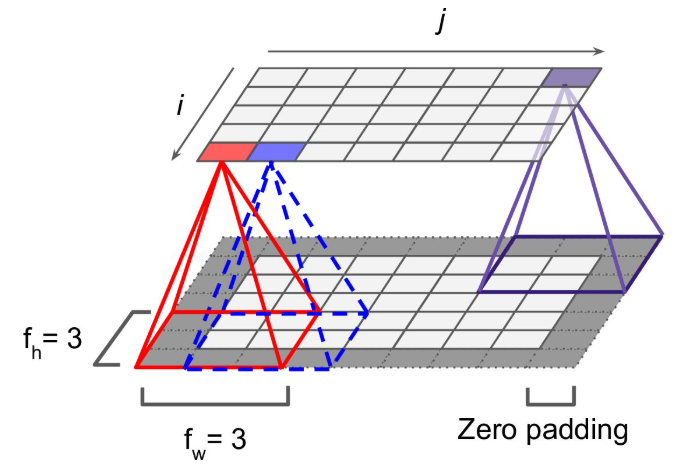
\includegraphics[width=0.72\textwidth]{./images/conv_layer.png}
\end{figure}

\newpage

\textbf{\underline{Filters and Feature Maps}}

A neuron's weights can be represented as a small image the size of the receptive field.\newline
These images are called \textit{filters} or \textit{convolutional kernels}.

It is common to apply the same filter to all neurons in a convolutional layer.\newline
The output is called a \textit{feature map}.\newline
It will highlight the areas in an image that activate the filter the most (e.g.~vertical lines).

In reality,
unlike the 2D diagram above,
a convolutional layer has multiple filters.\newline
This means it is more like a 3D object,
outputting one feature map per filter.

$\rightarrow$~A convolutional layer is capable of detecting multiple features
anywhere in its inputs.

\textit{Now consider the connections between 3D convolutional layers (or even to a RGB input):}\newline
A neuron located in row $i$, column $j$, feature map $k$, layer $l$ connects to...\newline
neurons in layer $l-1$, for the corresponding rows and columns, \textbf{across all feature maps}.

$\rightarrow$~You should now think of filters as 3D objects.\newline
$\rightarrow$~This means the weights of a convolutional layer are a 4D object.

Creating a convolutional layer in Keras:\newline
\texttt{conv = keras.layers.Conv2D(filters=32, kernel\char`_size=3, strides=1,\newline
.~~~~~~~~~~~~~~~~~~~~~~~~~~padding=\textquotesingle same\textquotesingle, activation=\textquotesingle relu\textquotesingle)}

When \texttt{padding=\textquotesingle same\textquotesingle}
the convolutional layer uses zero padding if necessary.\newline
When \texttt{padding=\textquotesingle valid\textquotesingle}
there is no zero padding (all receptive fields valid inside input).\newline\newline

\textbf{\underline{Pooling Layers}}

The goal of a \textit{pooling layer} is to subsample (i.e.~shrink) the input image.\newline
This reduces the computational load, the memory usage, and the number of parameters.\newline
The downside is that it is obviously very destructive.

Like in a convolutional layer,
each neuron in a pooling layer is connected to the outputs of a limited number of neurons in the previous layer.
You must define its kernel size, stride, and padding type.
Unlike a convolutional layer, a pooling neuron has no weights,
all it does is aggregate the inputs (it is most common to take the max).
A pooling layer typically works on every input channel independently,
so the output depth is the same as the input depth.

Creating a max pooling layer:\newline
\texttt{max\char`_pool = keras.layers.MaxPool2D(pool\char`_size=2)}\newline
By default, the stride is set to the kernel size and padding is set to `valid'.\newline

A \textit{global average pooling layer} computes the mean of each entire feature map.\newline
Although this is extremely destructive,
it can be useful as the output layer:\newline
\texttt{global\char`_average\char`_pool = keras.layers.GlobalAvgPool2D()}

\newpage
\textbf{\underline{CNN Architectures}}

Typical CNN architectures stack a few convolutional layers (each with a ReLU activation),
then a pooling layer, then another few convolutional layers, then another pooling layer, and so on.

$\rightarrow$ As it progresses through the network, the image gets smaller and smaller,
but also deeper and deeper (i.e~it has more feature maps).
This makes sense, since the number of low-level features is often fairly low,
but there are many different ways to combine them into higher-level features.

At the top of the stack,
a regular feed-forward neural network is added, composed of a few fully connected layers.
The final layer outputs the prediction.\newline

An example of a simple CNN to tackle the Fashion MNIST dataset:\newline
% 
\texttt{model = keras.models.Sequential([\newline
.~~~keras.layers.Conv2D(64, 7, activation=\textquotesingle relu\textquotesingle, padding=\textquotesingle same\textquotesingle,\newline
.~~~~~~~~~~~~~~~~~~~~~~~input\char`_shape=[28, 28, 1]),\newline
.~~~keras.layers.MaxPooling2D(2),\newline
.~~~keras.layers.Conv2D(128, 3, activation=\textquotesingle relu\textquotesingle, padding=\textquotesingle same\textquotesingle),\newline
.~~~keras.layers.Conv2D(128, 3, activation=\textquotesingle relu\textquotesingle, padding=\textquotesingle same\textquotesingle),\newline
.~~~keras.layers.MaxPooling2D(2),\newline
.~~~keras.layers.Conv2D(256, 3, activation=\textquotesingle relu\textquotesingle, padding=\textquotesingle same\textquotesingle),\newline
.~~~keras.layers.Conv2D(256, 3, activation=\textquotesingle relu\textquotesingle, padding=\textquotesingle same\textquotesingle),\newline
.~~~keras.layers.MaxPooling2D(2),\newline
.~~~keras.layers.Flatten(),\newline
.~~~keras.layers.Dense(128, activation=\textquotesingle relu\textquotesingle),\newline
.~~~keras.layers.Dropout(0.5),\newline
.~~~keras.layers.Dense(64, activation=\textquotesingle relu\textquotesingle),\newline
.~~~keras.layers.Dropout(0.5),\newline
.~~~keras.layers.Dense(10, activation=\textquotesingle softmax\textquotesingle)\newline
])}\newline

\textbf{Notes:}

A common mistake is to use convolutional kernels that are too large.
For example, instead of using a convolutional layer with a 5$\times$5 kernel,
stack two layers with 3$\times$3 kernels:
it will use fewer parameters and require fewer computations.
One exception is the first convolutional layer;
because the input images will only have 1 or 3 channels,
it can handle a larger kernel.

Because the input images are not very large, we do not set a stride in the model above.

It is common practice to double the number of filters after each pooling layer:
since a pooling layer divides each spatial dimension by a factor of 2,
we can afford to double the number of feature maps in the next layer
without exploding the number of parameters, memory usage, or computational load.

This model repeats the same structure twice:
two convolutional layers followed by a max pooling layer.
For larger images, we could repeat this structure several more times...

\newpage
\textbf{\underline{ResNet (Residual Network)}}

ResNet is a state of the art image classifier.
It is very deep, some variants have over 100 layers.

The key to training such a deep network is to use \textit{skip connections} (or \textit{shortcut connections}):\newline
the signal feeding into a layer is also added to the output of a layer located higher up the stack.

If you use a skip connection,
the network will be forced to model $f(\boldsymbol{x}) = h(\boldsymbol{x}) - \boldsymbol{x}$
\newline rather than $h(\boldsymbol{x})$.
This is called \textit{residual learning} (hence ResNet's name). Positives:\newline
- At the start of training (when weights are small), skip connections model the identity function.\newline
- Also, the network can start making progress even if several layers have not started learning.

ResNet can be seen as a deep stack of \textit{residual units (RUs)},
where each RU is a small neural network with a skip connection.
Below is a diagram of the ResNet architecture.
Note that $64,~7\!\times\!7 + 2(\textrm{S})$ represents 64 feature maps,
using a $7\!\times\!7$ kernel, with stride 2 (using `same' padding):

\begin{figure}[ht]
\centering
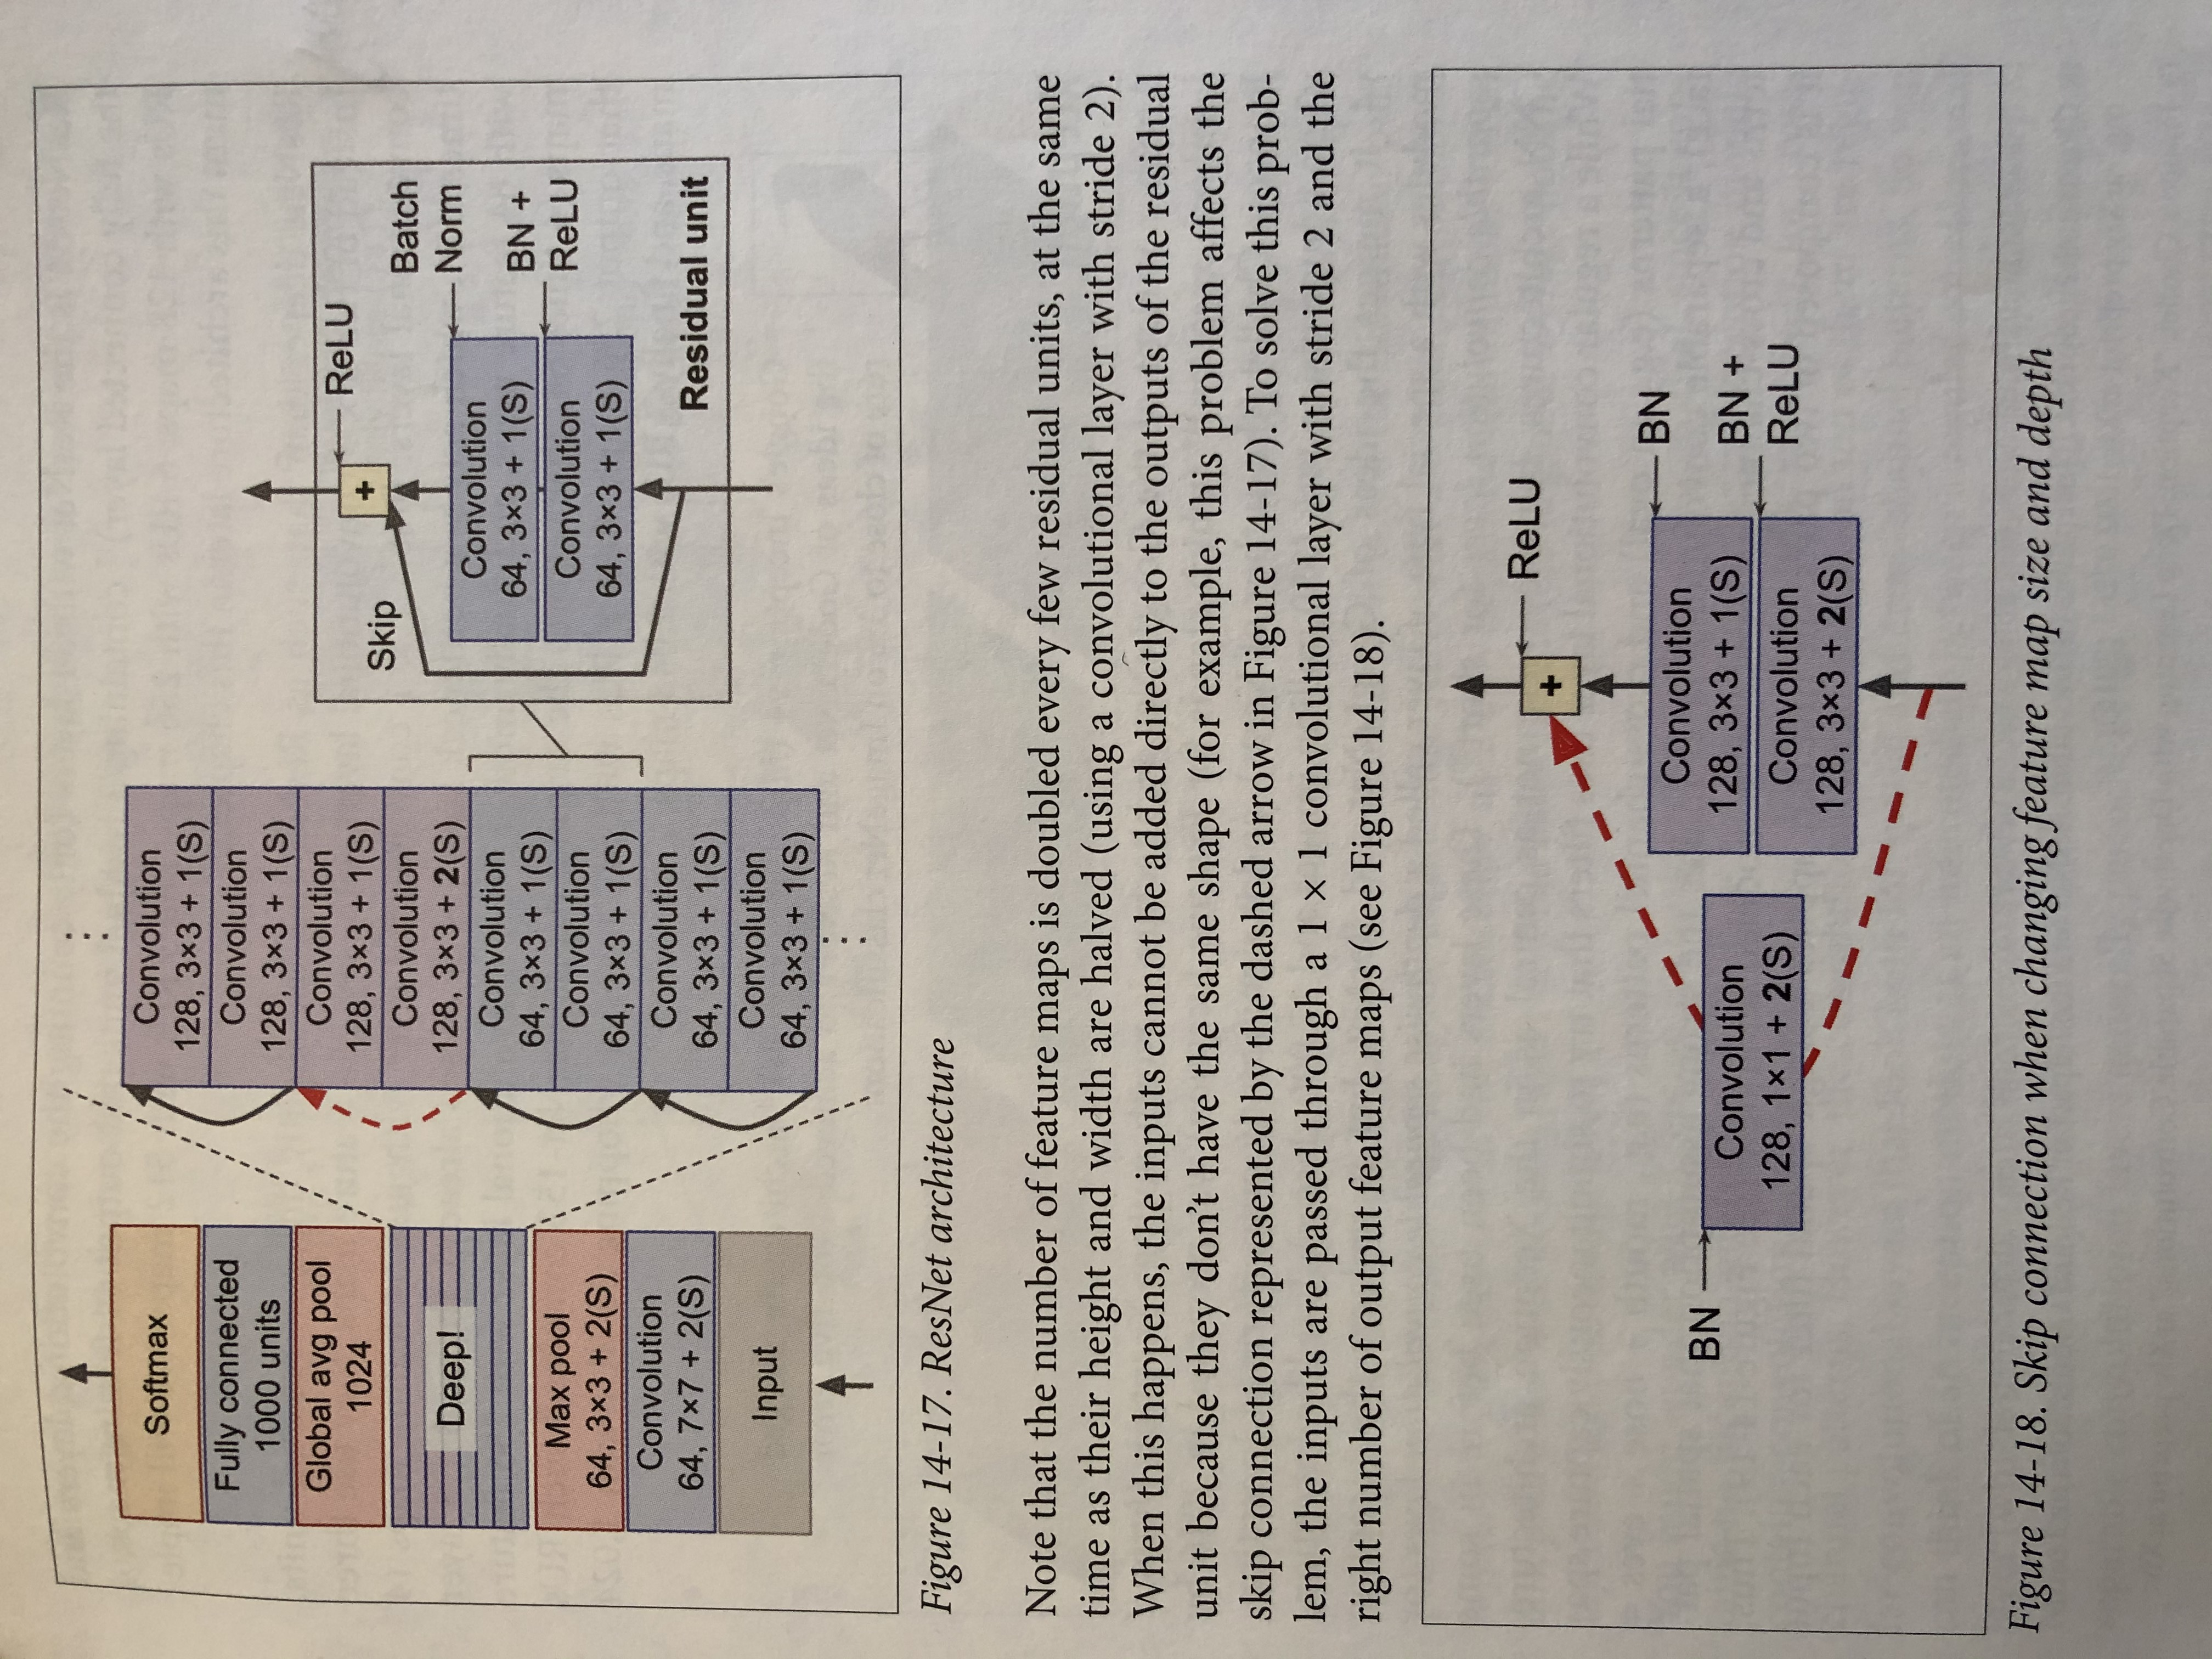
\includegraphics[width=1.0\textwidth, angle=270]{./images/resnet.jpg}
\end{figure}

\newpage
ResNet-34 is the ResNet with 34 layers (only counting convolutional layers and fully connected layers).
It contains 3 RUs with 64 maps, 4 RUs with 128 maps, 6 RUs with 256 maps, and 3~RUs with 512 maps.
It can be implemented from scratch using Keras:

\texttt{class ResidualUnit(keras.layers.Layer):}\newline
\texttt{.~~~def \char`_\char`_init\char`_\char`_(self, filters, strides=1, activation=\textquotesingle relu\textquotesingle, **kwargs):}\newline
\texttt{.~~~~~~~super().\char`_\char`_init\char`_\char`_(**kwargs)}\newline
\texttt{.~~~~~~~self.activation = keras.activations.get(activation)}\newline
\texttt{.~~~~~~~self.main\char`_layers = [}\newline
\texttt{.~~~~~~~~~~~keras.layers.Conv2D(filters, 3, strides=strides,}\newline
\texttt{.~~~~~~~~~~~~~~~~~~~~~~~~~~~~~~~padding=\textquotesingle same\textquotesingle, use\char`_bias=False),}\newline
\texttt{.~~~~~~~~~~~keras.layers.BatchNormalization(),}\newline
\texttt{.~~~~~~~~~~~self.activation,}\newline
\texttt{.~~~~~~~~~~~keras.layers.Conv2D(filters, 3, strides=1,}\newline
\texttt{.~~~~~~~~~~~~~~~~~~~~~~~~~~~~~~~padding=\textquotesingle same\textquotesingle, use\char`_bias=False),}\newline
\texttt{.~~~~~~~~~~~keras.layers.BatchNormalization()]}\newline
\texttt{.~~~~~~~self.skip\char`_layers = []}\newline
\texttt{.~~~~~~~if strides > 1:}\newline
\texttt{.~~~~~~~~~~~self.skip\char`_layers = [}\newline
\texttt{.~~~~~~~~~~~~~~~keras.layers.Conv2D(filters, 1, strides=strides,}\newline
\texttt{.~~~~~~~~~~~~~~~~~~~~~~~~~~~~~~~~~~~padding=\textquotesingle same\textquotesingle, use\char`_bias=False),}\newline
\texttt{.~~~~~~~~~~~~~~~keras.layers.BatchNormalization()]}\newline
\texttt{}\newline
\texttt{.~~~def call(self, inputs):}\newline
\texttt{.~~~~~~~Z = inputs}\newline
\texttt{.~~~~~~~for layer in self.main\char`_layers:}\newline
\texttt{.~~~~~~~~~~~Z = layer(Z)}\newline
\texttt{.~~~~~~~skip\char`_Z = inputs}\newline
\texttt{.~~~~~~~for layer in self.skip\char`_layers:}\newline
\texttt{.~~~~~~~~~~~skip\char`_Z = layer(skip\char`_Z)}\newline
\texttt{.~~~~~~~return self.activation(Z + skip\char`_Z)}\newline

\texttt{model = keras.models.Sequential()}\newline
\texttt{model.add(keras.layers.Conv2D(64, 7, strides=2,}\newline
\texttt{.~~~~~~~~~~~~~~~~~~~~~~~~~~~~~input\char`_shape=[224, 224, 3],}\newline
\texttt{.~~~~~~~~~~~~~~~~~~~~~~~~~~~~~padding=\textquotesingle same\textquotesingle, use\char`_bias=False))}\newline
\texttt{model.add(keras.layers.BatchNormalization())}\newline
\texttt{model.add(keras.layers.Activation(\textquotesingle relu\textquotesingle))}\newline
\texttt{model.add(keras.layers.MaxPool2D(pool\char`_size=3, strides=2, padding=\textquotesingle same\textquotesingle))}\newline
\texttt{prev\char`_filters = 64}\newline
\texttt{for filters in [64] * 3 + [128] * 4 + [256] * 6 + [512] * 3:}\newline
\texttt{.~~~strides = 1 if filters == prev\char`_filters else 2}\newline
\texttt{.~~~model.add(ResidualUnit(filters, strides=strides))}\newline
\texttt{.~~~prev\char`_filters = filters}\newline
\texttt{model.add(keras.layers.GlobalAvgPool2D())}\newline
\texttt{model.add(keras.layers.Flatten())}\newline
\texttt{model.add(keras.layers.Dense(10, activation=\textquotesingle softmax\textquotesingle))}

\newpage
\textbf{\underline{Using Pre-trained Models}}

In general, you don't have to implement standard models manually:\newline
\texttt{model = keras.applications.resnet50.ResNet50(weights=\textquotesingle imagenet\textquotesingle)}

They are very easy to use...\newline
\texttt{from matplotlib.image import imread}\newline
\texttt{}\newline
\texttt{image\char`_01 = imread(\textquotesingle /path/to/file\char`_01.jpeg\textquotesingle)}\newline
\texttt{image\char`_01\char`_resized = tf.image.resize(image\char`_01, [224, 224])}\newline
\texttt{...}\newline
\texttt{image\char`_99 = imread(\textquotesingle /path/to/file\char`_99.jpeg\textquotesingle)}\newline
\texttt{image\char`_99\char`_resized = tf.image.resize(image\char`_99, [224, 224])}\newline
\texttt{}\newline
\texttt{images = tf.stack([image\char`_01\char`_resized, ..., image\char`_99\char`_resized])}\newline
\texttt{inputs = keras.applications.resnet50.preprocess\char`_input(images)}\newline
\texttt{Y\char`_proba = model.predict(inputs)}\newline
\texttt{}\newline
\texttt{top\char`_K = keras.applications.resnet50.decode\char`_predictions(Y\char`_proba, top=5)}\newline
\texttt{for info in top\char`_K: print(info); print()}\newline

\textbf{\underline{Transfer Learning}}

If you want to build an image classifier but you do not have enough training data,
then it is often a good idea to reuse the lower layers of a pre-trained model.

Load a dataset using TensorFlow Datasets:\newline
\texttt{import tensorflow\char`_datasets as tfds}\newline
\texttt{data, info = tfds.load(\textquotesingle tf\char`_flowers\textquotesingle, split=[\textquotesingle train[:70\%]\textquotesingle, \textquotesingle train[70\%:]\textquotesingle],}\newline
\texttt{.~~~~~~~~~~~~~~~~~~~~~~~with\char`_info=True, as\char`_supervised=True)}\newline
\texttt{train\char`_set, valid\char`_set = data[0], data[1]}\newline
\texttt{n\char`_classes = info.features[\textquotesingle label\textquotesingle].num\char`_classes}

Prepare the datasets:\newline
\texttt{def preprocess(image, label):}\newline
\texttt{.~~~resized\char`_im = tf.image.resize(image, [224, 224])}\newline
\texttt{.~~~final\char`_im = keras.applications.xception.preprocess\char`_input(resized\char`_im)}\newline
\texttt{.~~~return final\char`_im, label}

\texttt{train\char`_set = train\char`_set.shuffle(1000)}\newline
\texttt{train\char`_set = train\char`_set.map(preprocess).batch(32).prefetch(1)}\newline
\texttt{valid\char`_set = valid\char`_set.map(preprocess).batch(32).prefetch(1)}

Load a pre-trained Xception model (excluding the top of the network) and add a custom top:\newline
\texttt{base\char`_model = keras.applications.xception.Xception(weights=\textquotesingle imagenet\textquotesingle,\newline
.~~~~~~~~~~~~~~~~~~~~~~~~~~~~~~~~~~~~~~~~~~~~~~~~~include\char`_top=False)}\newline
\texttt{avg = keras.layers.GlobalAveragePooling2D()(base\char`_model.output)}\newline
\texttt{output = keras.layers.Dense(n\char`_classes, activation=\textquotesingle softmax\textquotesingle)(avg)}\newline
\texttt{model = keras.Model(inputs=base\char`_model.input, outputs=output)}

Freeze the weights of the pre-trained layers at the beginning of training:\newline
\texttt{for layer in base\char`_model.layers:}\newline
\texttt{.~~~layer.trainable = False}

\texttt{optimizer = keras.optimizers.SGD(lr=0.2, momentum=0.9, decay=0.01)}\newline
\texttt{model.compile(loss=\textquotesingle sparse\char`_categorical\char`_crossentropy\textquotesingle, optimizer=optimizer,\newline
.~~~~~~~~~~~~~metrics=[\textquotesingle accuracy\textquotesingle])}\newline
\texttt{save\char`_cb = keras.callbacks.ModelCheckpoint(\textquotesingle flower\char`_classifier.h5\textquotesingle,}\newline
\texttt{.~~~~~~~~~~~~~~~~~~~~~~~~~~~~~~~~~~~~~~~~~~save\char`_best\char`_only=True)}\newline
\texttt{history = model.fit(train\char`_set, epochs=5, validation\char`_data=valid\char`_set,}\newline
\texttt{.~~~~~~~~~~~~~~~~~~~callbacks=[save\char`_cb])}

When the top layers are well trained, unfreeze all the layers and continue training\newline
(this time using a much lower learning rate to avoid damaging the pre-trained weights):\newline
\texttt{model = keras.models.load\char`_model(\textquotesingle flower\char`_classifier.h5\textquotesingle)}

\texttt{for layer in model.layers:}\newline
\texttt{.~~~layer.trainable = True}

\texttt{optimizer = keras.optimizers.SGD(lr=0.01, momentum=0.9, decay=0.001)}\newline
\texttt{model.compile(...) \# always compile models after (un)freezing layers}\newline
\texttt{history = model.fit(...)}

%%%%%%%%%%%%%%%%%%%%%%%%%%%
%%%%%%%%%%%%%%%%%%%%%%%%%%%
%%%%%%%%%%%%%%%%%%%%%%%%%%%
%%%%%%%%%%%%%%%%%%%%%%%%%%%
%%%%%%%%%%%%%%%%%%%%%%%%%%%
\subsection{Processing Sequences Using RNNs}

Recurrent neural networks (RNNs) are a class of nets that can predict the future.\newline
They can work on sequences of arbitrary lengths, rather than on fixed-sized inputs.\newline
RNNs look a lot like feedforward NNs,
except they also have connections pointing backward.\newline

\textbf{\underline{Recurrent Neurons}}

A single recurrent neuron is the simplest possible RNN.
At each \textit{timestep t} (also called a \textit{frame}),
it receives inputs $\boldsymbol{x}_{(t)}$ as well as it's own output from the previous step, $y_{(t-1)}$.
Since there is no previous output at the first time step, it is generally set to 0.
The following diagram unrolls the network through time (note that it is the \underline{same} neuron represented once per timestep).

\begin{figure}[ht]
\centering
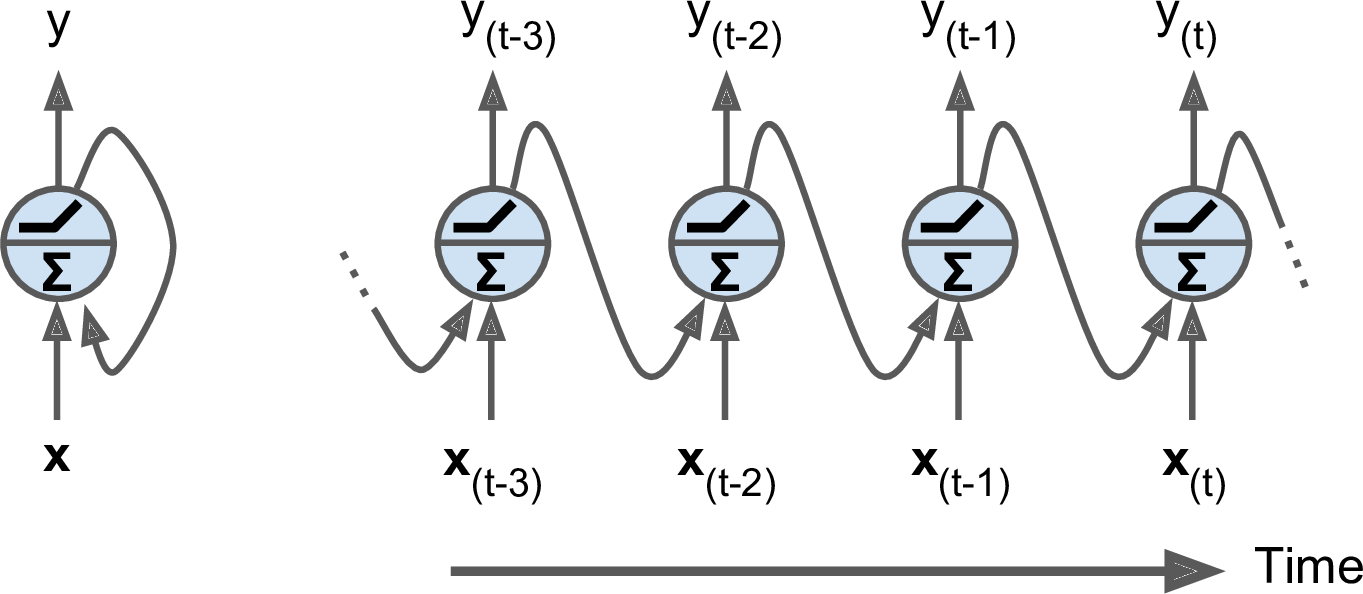
\includegraphics[width=0.80\textwidth]{./images/recurrent_neuron.png}
\end{figure}

\newpage
\textbf{\underline{Recurrent Layers}}

It is easy to extend the concept described above to create a layer of recurrent neurons.\newline
At each timestep $t$, \underline{every} neuron receives both the input vector $\boldsymbol{x}_{(t)}$
and the output vector\newline from the previous timestep $\boldsymbol{y}_{(t-1)}$.
This output vector is formed from each neurons scalar output.

Each recurrent neuron has two sets of weights: one for $\boldsymbol{x}_{(t)}$ and another for $\boldsymbol{y}_{(t-1)}$:\newline
$y^{(t)}_i = \phi (w^x_{ij} \: x^{(t)}_j + w^y_{ij} \: y^{(t-1)}_j + b_i)$

Note that the full sequence $\boldsymbol{x}_{(t)}$ is just a single training instance.\newline

\textbf{\underline{Memory Cells}}

Since the output of a recurrent neuron at timestep $t$ is a function of all the inputs from previous timesteps,
you could say it has a form of \textit{memory}.
A part of a neural network that preserves some state across timesteps is called a \textit{memory cell}.
% 
A single layer of recurrent neurons is a very basis memory cell,
capable of learning only short patterns (typically 10 steps long).

In general, a cell's (hidden) state at timestep $t$ is:~~~~~~$\boldsymbol{h}_{(t)} = f(\boldsymbol{h}_{(t-1)}, \boldsymbol{x}_{(t)})$\newline
This is not necessarily the same as the cell's output: $\boldsymbol{y}_{(t)} = g(\boldsymbol{h}_{(t-1)}, \boldsymbol{x}_{(t)})$\newline

\begin{figure}[ht]
\centering
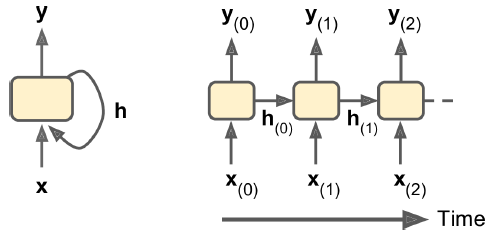
\includegraphics[width=0.80\textwidth]{./images/memory_cells.png}
\end{figure}

\vspace{+4.0mm}
\textbf{\underline{Training RNNs}}

To train an RNN, the trick is to unroll it through time and then simply use regular backpropagation.
This strategy is called \textit{backpropagation through time} (BPTT).
Fortunately, Keras takes care of all the complexity for us!\newline

\textbf{\underline{Forecasting a Time Series}}

A time series is a sequence of one or more values per timestep.\newline
\textit{Univariate time series} = single value per timestep.\newline
\textit{Multivariate time series} = multiple values per timestep.

A typical task is to predict future values, which is called \textit{forecasting}.\newline
Filling in missing values from the past is called \textit{imputation}.

\newpage

Time series are represented as 3D arrays of shape [\textit{batch-size, timesteps, value dimensionality}]

\texttt{def generate\char`_time\char`_series(batch\char`_size, n\char`_steps):}\newline
\texttt{.~~~freq1,freq2,offset1,offset2 = np.random.rand(4, batch\char`_size, 1)}\newline
\texttt{.~~~time = np.linspace(0, 1, n\char`_steps)}\newline
\texttt{.~~~series = 0.5 * np.sin((time - offset1) * (freq1 * 10 + 10))}\newline
\texttt{.~~~series += 0.2 * np.sin((time - offset2) * (freq2 * 20 + 20))}\newline
\texttt{.~~~series += 0.1 * (np.random.rand(batch\char`_size, n\char`_steps) - 0.5)}\newline
\texttt{.~~~return series[..., np.newaxis].astype(np.float32)}\newline

Let's create a model to forecast the value at the next timestep of 1000's of these timeseries:\newline
\texttt{n\char`_steps = 50}\newline
\texttt{series = generate\char`_time\char`_series(10000, n\char`_steps + 1)}

Use 75\% of data for training and 25\% for validation.
Input the first 50 steps and target the final step. (Note that the target will shape what the model is trying to do).\newline
\texttt{train\char`_X = series[:7500, :n\char`_steps]}\newline
\texttt{train\char`_y = series[:7500, -1]}\newline
\texttt{valid\char`_X = series[7500:, :n\char`_steps]}\newline
\texttt{valid\char`_y = series[7500:, -1]}\newline

Create a \textit{naive forecasting} baseline metric (predict the last value in each series):\newline
\texttt{valid\char`_pred\char`_y = valid\char`_X[:, -1]}\newline
\texttt{np.mean(keras.losses.mean\char`_squared\char`_error(valid\char`_y, valid\char`_pred\char`_y))}\newline

Implement a Simple RNN:\newline
\texttt{model = keras.models.Sequential()}\newline
\texttt{model.add(keras.layers.SimpleRNN(1, input\char`_shape=[None, 1]))}

- It just contains a single layer, with a single neuron (it only has three parameters).\newline
- By default, it uses the hyperbolic tangent activation function.\newline
- The first input dimension is set to `None', as it can process any number of timesteps.\newline
- By default, recurrent layers in Keras only return the final output.\newline
- To return one output per timestep, set \texttt{return\char`_sequences=True}

Compile, fit, and evaluate:\newline
\texttt{model.compile(loss=\textquotesingle mean\char`_squared\char`_error\textquotesingle, optimizer=\textquotesingle Adam\textquotesingle)}\newline
% \texttt{early\char`_stop\char`_cb = keras.callbacks.EarlyStopping(patience=10, restore\char`_best\char`_weights=True)}\newline
\texttt{model.fit(train\char`_X, train\char`_y, epochs=50,\newline
.~~~~~~~~~validation\char`_data=(valid\char`_X, valid\char`_y), callbacks=[early\char`_stop\char`_cb])}

\texttt{valid\char`_pred\char`_y = model.predict(valid\char`_X)}\newline
\texttt{np.mean(keras.losses.mean\char`_squared\char`_error(valid\char`_y, valid\char`_pred\char`_y))}

\newpage
\textbf{\underline{Deep RNNs}}

It is common to stack multiple layers of cells, giving you a \textit{Deep RNN}.\newline

\begin{figure}[ht]
\centering
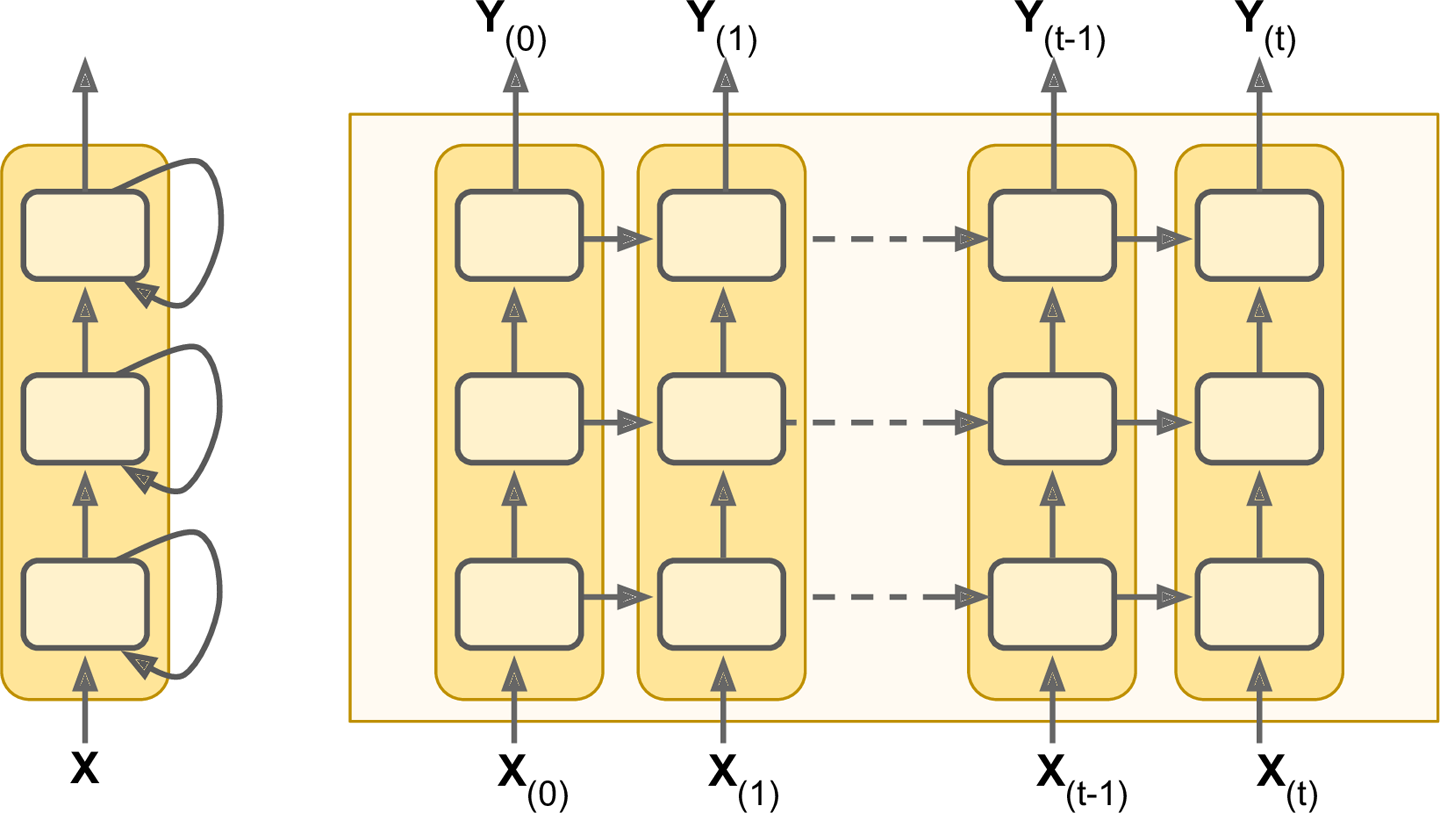
\includegraphics[width=0.75\textwidth]{./images/deep_RNN.png}
\end{figure}

\vspace{+4.0mm}
\texttt{model = keras.models.Sequential([}\newline
\texttt{keras.layers.SimpleRNN(20, return\char`_sequences=True, input\char`_shape=[None,1]),}\newline
\texttt{keras.layers.SimpleRNN(20, return\char`_sequences=True),}\newline
\texttt{keras.layers.SimpleRNN(1)}\newline
\texttt{])}

Note that sometimes it might be preferable to replace the output layer with a Dense layer.\newline

\textbf{\underline{Unstable Gradients Problem}}

To train an RNN on long sequences, we must run it over many time steps, making the unrolled RNN a very deep network.    
Consequently, it may suffer from the unstable gradients problem:

\vspace{-3.5mm}
\begin{itemize}
\item
Due to the architecture of RNNs, they are more likely to suffer from exploding outputs and exploding gradients (rather than vanishing gradients).
\item
\vspace{-2.0mm}
Consequently, saturating activation functions (e.g. hyperbolic tangent) are recommended.
\item
\vspace{-2.0mm}
Batch Normalization doesn't really work, but the \textit{Layer Normalization} technique might.
\end{itemize}


\textbf{\underline{Short-Term Memory Problem}}

When an RNN processes a long sequence, it will gradually forget the first inputs in the sequence.
The cells we've looked at so far have a very short memory (about 10 timesteps).
To tackle this, more complex cells with longer memory (about 100 steps) have been successfully introduced.
These are the \textit{Long Short-Term Memory} (LSTM) cell and the \textit{Gated Recurrent Unit} GRU cell.

\texttt{keras.layers.LSTM(20, return\char`_sequences=True)}\newline
or\newline
\texttt{keras.layers.GRU(20, return\char`_sequences=True)}

Note that there is also some cool stuff combining 1D convolutional layers with RNNs.

\newpage

\textbf{\underline{Input and Output Sequences}}

Our forecasting model was a \textit{sequence-to-vector} network (ignore all outputs except the last).
% 
E.g.~you feed it a value at 50 timesteps and it will predict the value for the next 10 timesteps.\newline
E.g.~you feed it a sequence of words from a movie review and it will predict a semantic score.

A \textit{sequence-to-sequence} network returns all the outputs.\newline
E.g.~forecast the next 10 values at each and every timestep.
The advantage of this technique is that the loss will contain a term for the output of the RNN at each timestep,
creating many more error gradients flowing through the model,
which stabilizes and speeds up training.

The \texttt{TimeDistributed} layer allows you to wrap \underline{any} layer and apply it at every timestep:\newline
\texttt{model = keras.models.Sequential([}\newline
\texttt{keras.layers.LSTM(20, return\char`_sequences=True, input\char`_shape=[None,1]),}\newline
\texttt{keras.layers.LSTM(20, return\char`_sequences=True),}\newline
\texttt{keras.layers.TimeDistributed(keras.layers.Dense(10))}\newline
\texttt{])}

Note that preparing the target now becomes a bit more of a headache!

%%%%%%%%%%%%%%%%%%%%%%%%%%%
%%%%%%%%%%%%%%%%%%%%%%%%%%%
%%%%%%%%%%%%%%%%%%%%%%%%%%%
%%%%%%%%%%%%%%%%%%%%%%%%%%%
%%%%%%%%%%%%%%%%%%%%%%%%%%%
\subsection{Autoencoders}

Autoencoders are neural networks capable of learning dense representations of the input data,
called \textit{latent representations} or \textit{codings}, without any supervision. They are useful for:
\vspace{-3.5mm}
\begin{itemize}
\item
Dimensionality reduction.
\item
\vspace{-2.0mm}
Unsupervised pretraining of DNNs.
\item
\vspace{-2.0mm}
Generative models (randomly generating new data that looks like the training data).
\end{itemize}

\vspace{-2.5mm}
Autoencoders simply learn to copy their inputs to their outputs.
This may sound trivial,
but you would typically limit the size of the latent representation
or try to recover the original inputs after adding some noise,
forcing the autoencoder to learn efficient ways of representing the data.

Autoencoders are always composed of two parts:\newline
- An \textit{encoder} (or \textit{recognition network}) that converts the inputs into a latent representation.\newline
- A \textit{decoder} (or \textit{generative network}) that converts the internal representation into the outputs.\newline

\begin{figure}[ht]
\centering
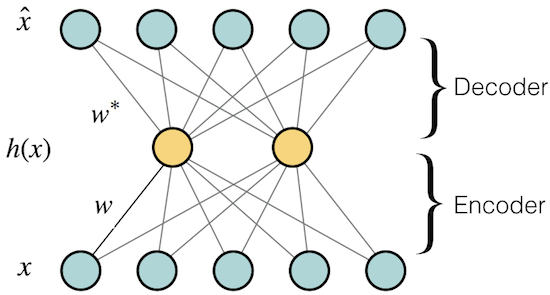
\includegraphics[width=0.60\textwidth]{./images/autoencoder.png}
\end{figure}

\texttt{encoder = keras.models.Sequential([keras.layers.Dense(2,input\char`_shape=[5])])}\newline
\texttt{decoder = keras.models.Sequential([keras.layers.Dense(5,input\char`_shape=[2])])}\newline
\texttt{autoencoder = keras.models.Sequential([encoder, decoder])}

\texttt{autoencoder.compile(loss=\textquotesingle mse\textquotesingle, optimizer=keras.optimizers.SGD(lr=0.1))}\newline
\texttt{history = autoencoder.fit(train\char`_X, train\char`_X, epochs=20)}\newline
\texttt{codings = encoder.predict(train\char`_X)}

Autoencoders with multiple hidden layers are called \textit{stacked} or \textit{deep autoencoders}.
The architecture is typically symmetrical with respect to the central hidden layer (the coding layer).
Note that this can be achieved for both CNN and RNN models (see the examples in the textbook).

One way to ensure that an autoencoder is properly trained is to compare the inputs and the outputs from the validation set: the differences should not be too significant.
Note that if you make the network too powerful, it will manage to make perfect reconstructions on the training data without having learned any useful patterns
(and is unlikely to generalize well to new instances).

Autoencoders make it possible to perform \textit{semantic interpolation}:\newline
Instead of interpolating two images at the pixel level (which would look as if the two images were overlaid),
we can interpolate at the codings level.\newline
- First, run both images through the encoder.\newline
- Next, interpolate the two codings.\newline
- Finally, decode the interpolated coding to get the final image.\newline
- Note that you can do all sorts of arithmetic in latent space!\newline

\textbf{\underline{Unsupervised Pretraining}}

If you have a large dataset but most of it is unlabeled,
you can first train a stacked autoencoder using all the data,
then reuse the lower layers to create a neural network for your actual task (and train it using the labeled data).

\begin{figure}[ht]
\centering
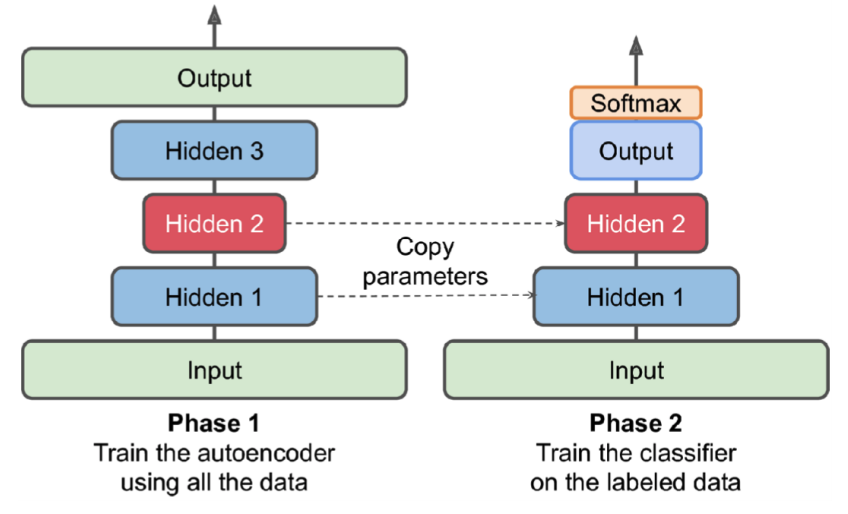
\includegraphics[width=0.80\textwidth]{./images/unsupervised_pretraining.png}
\end{figure}

%%%%%%%%%%%%%%%%%%%%%%%%%%%
%%%%%%%%%%%%%%%%%%%%%%%%%%%
%%%%%%%%%%%%%%%%%%%%%%%%%%%
%%%%%%%%%%%%%%%%%%%%%%%%%%%
%%%%%%%%%%%%%%%%%%%%%%%%%%%
\subsection{Generative Adversarial Networks (GANs)}

GANs are composed of two neural networks that compete against each other during training.

The \textit{Generator}:\newline
Takes a random distribution as the input (typically Gaussian) and outputs some data.
Its goal is to generate data that looks similar to the training data.
You can think of the random inputs as the latent representations and the generator as a decoder.
Once it is trained, you can feed the generator some Gaussian noise and it will output a brand-new `image'.

The \textit{Discriminator}:\newline
Takes either a fake image from the generator or a real image from the training set as an input,
and must guess whether the image is fake or real.\newline

\begin{figure}[ht]
\centering
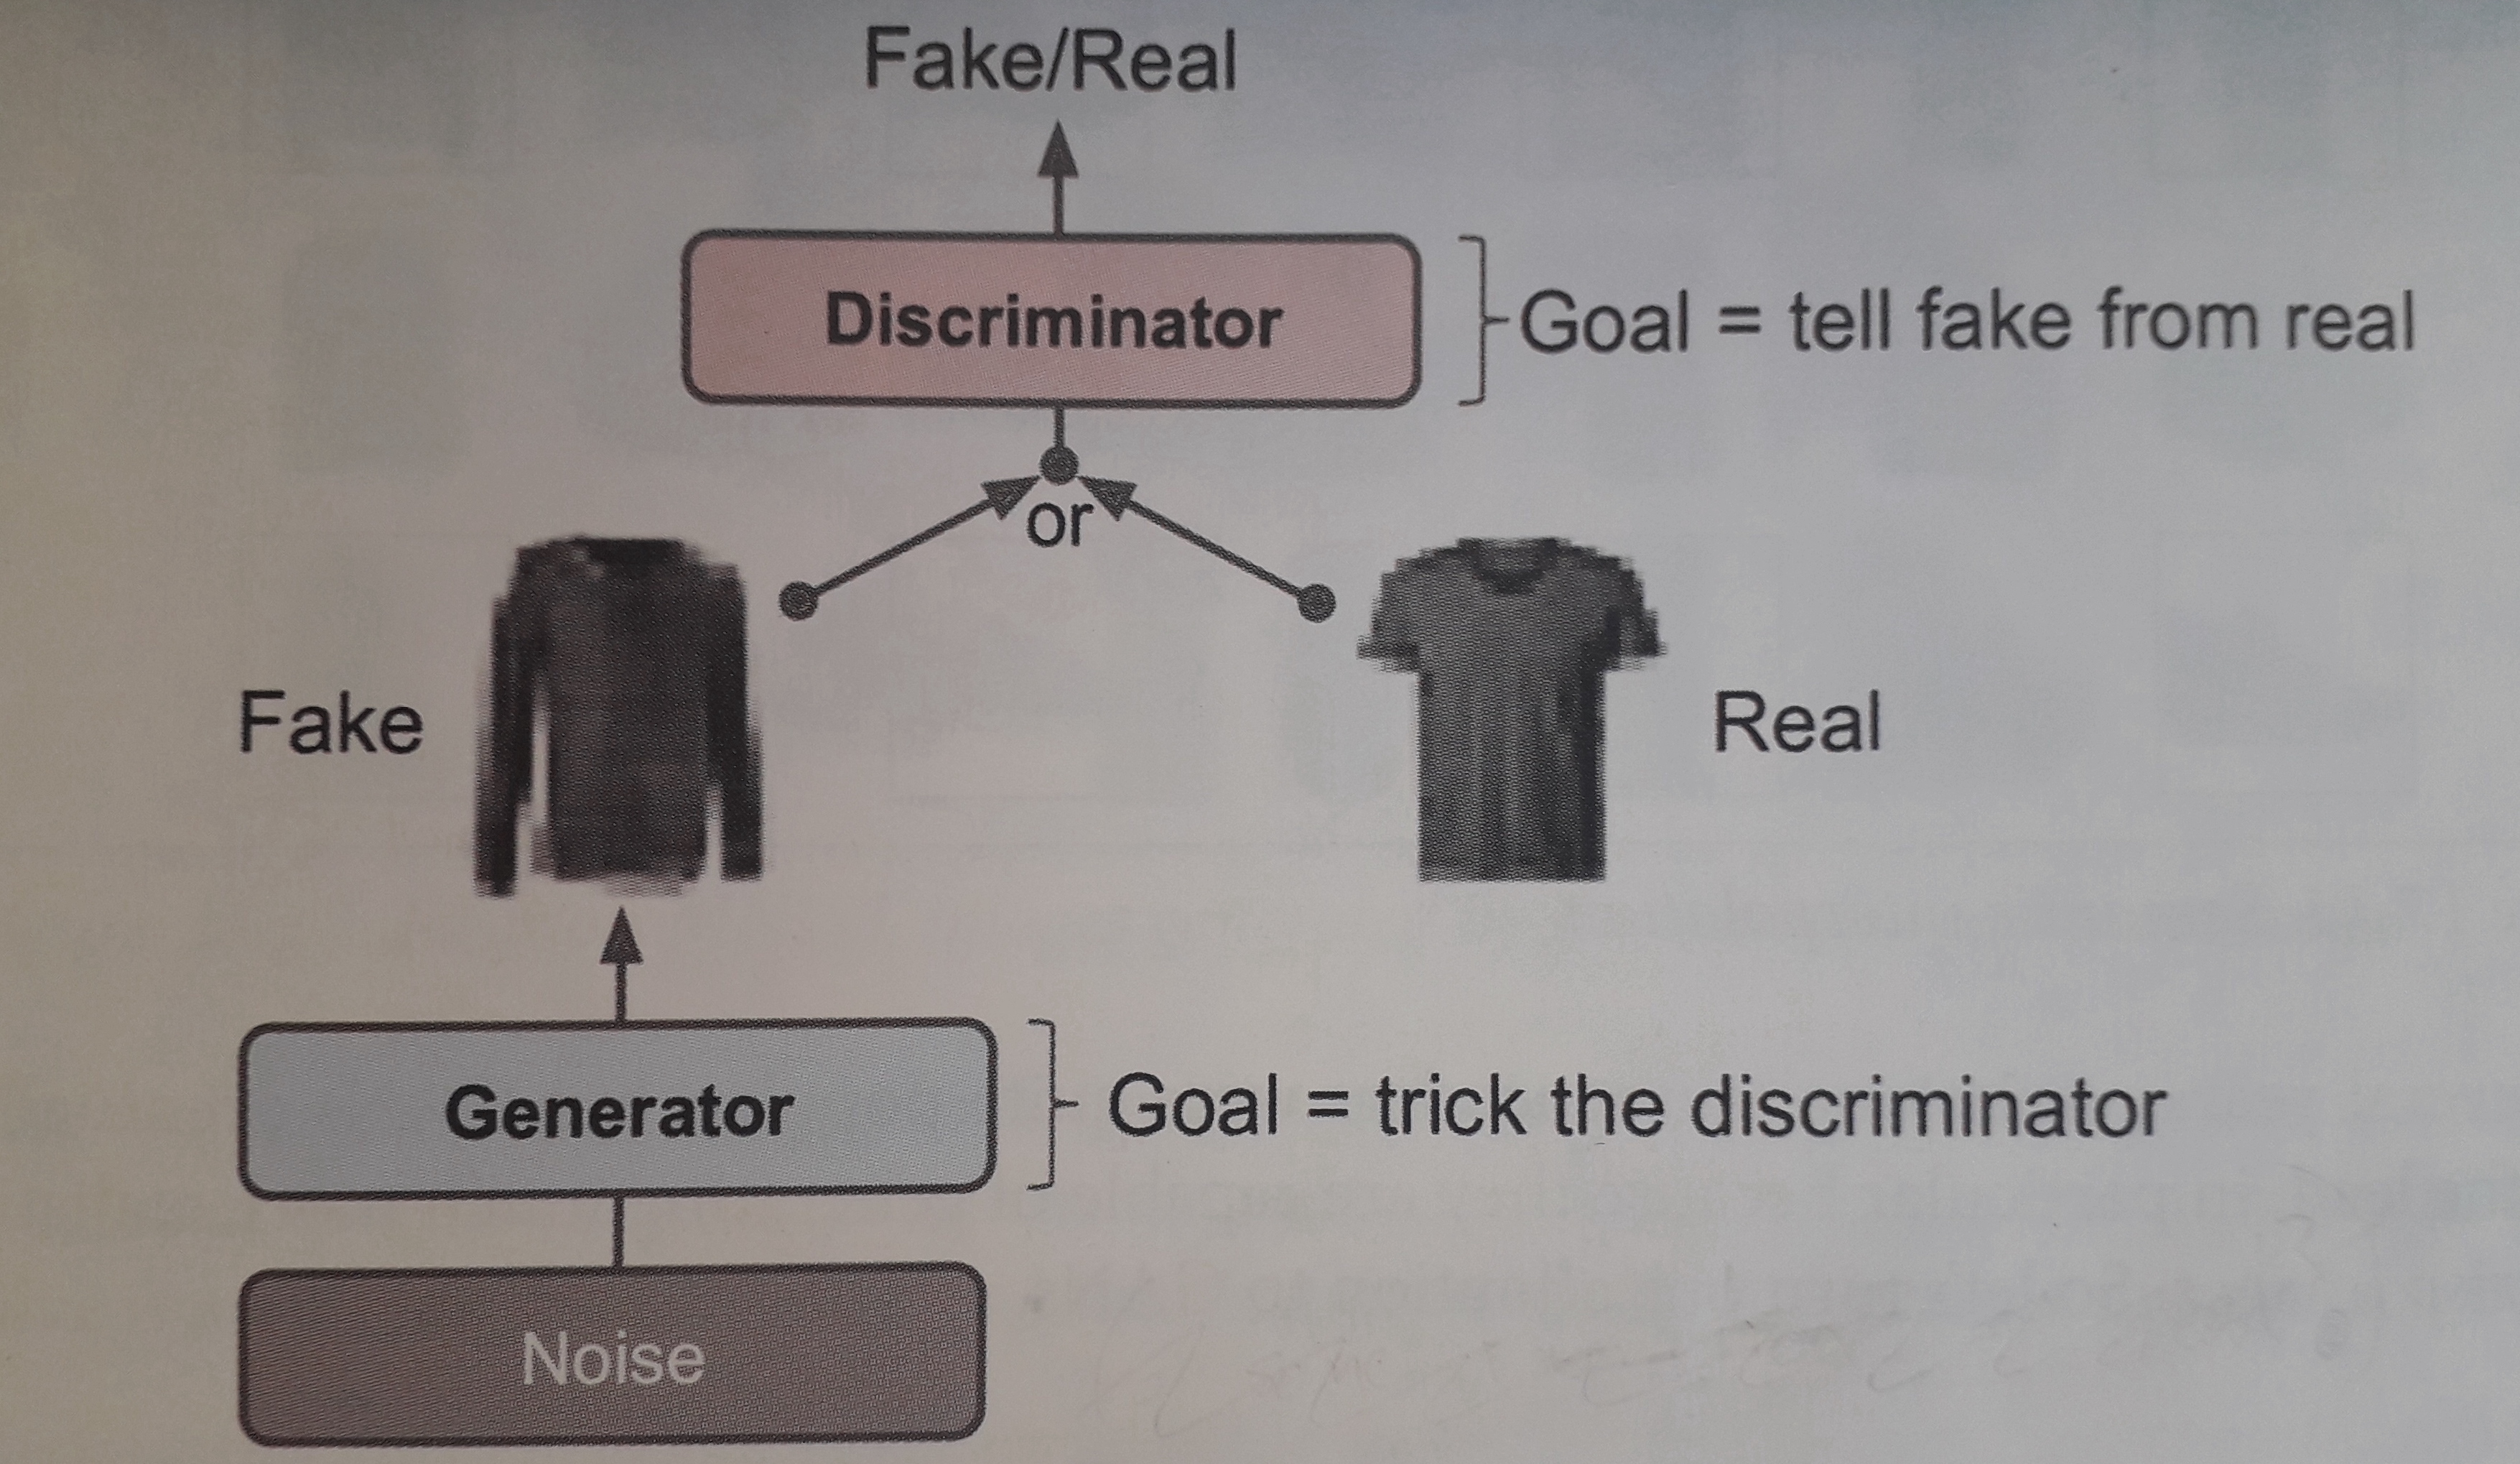
\includegraphics[width=0.80\textwidth]{./images/gan.jpg}
\end{figure}



\newpage